\documentclass{dalthesis}

\usepackage{float}
\usepackage{graphicx}
\usepackage{listings}

\graphicspath{ {./images/} }

\begin{document}

\author{Utku Gultopu}
\mcs

\mainmatter

\chapter{Approach}

We start by selecting an image that has the potential to be a good candidate for constructing a level. This potential is primarily determined by the shape of the outline of the object represented by the image, as the content, lighting, coloring, resolution, size and even format is not of any concern of us for the purposes of generating a level. This is because the only use of the input image, the raster image, for us is to convert the input image into a vector image, specifically a Scalable Vector Graphics (SVG) image, before executing the code that actually generates a Science Birds structure. Since this code operates on an SVG image, specifically an SVG image with a \lstinline{polygon} element, all the operation that we do before feeding an SVG image that contains a \lstinline{polygon} element to the code can be simply understood as the "preprocessing stage" for constructing a Science Birds structure. Nevertheless, in order to start with a raster image and attain a Science Birds structure, all the steps in the preprocessing stage are necessary. These steps can be listed as follows:

\begin{figure}[H]
  \centering
  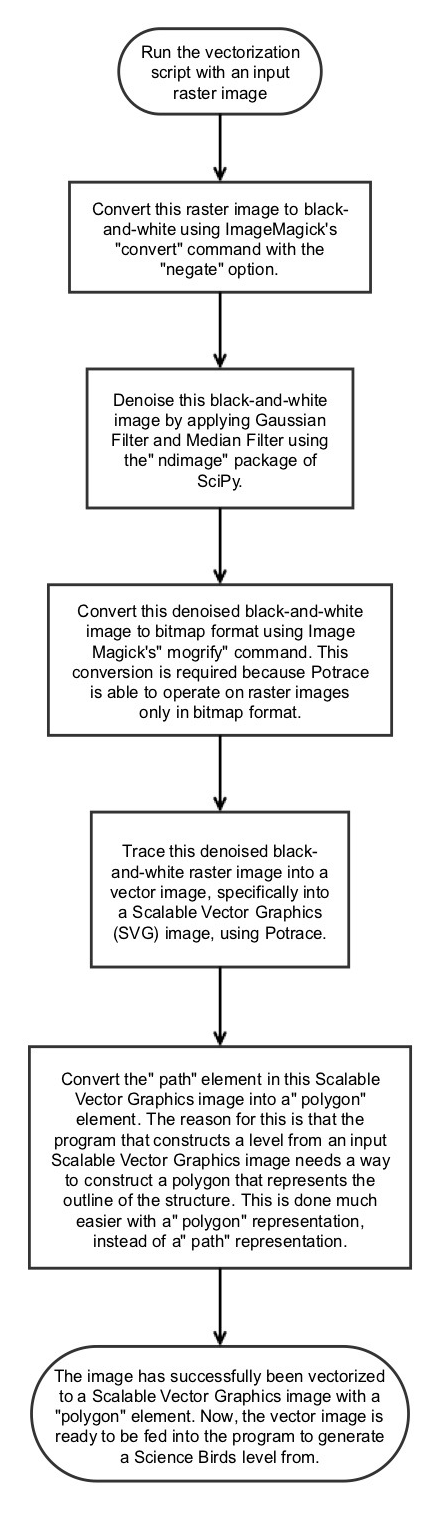
\includegraphics[width=\textwidth,height=\textheight,keepaspectratio]{process/science_birds_pcg-raster_to_vector-edited.png}
\end{figure}

Some of the steps in the flowchart are explained in detail below:

\begin{enumerate}
  \item Converting a raster image to black-and-white: The reason for this is actually clear. We have stated that the content, lighting, coloring, resolution size or format of the image is of no concern to us, as we have stated that the only use of the image is the outline of the structure represented in that image. We have also stated that the raster image, for the purposes of generating a Science Birds structure is of no use to us, since it is not possible (or, straightforward) to obtain the outline data of the image from the raster image. Since that's the case, content, lighting and similar are simply redundant information for all of our purposes. Hence, in order to have an easier and more precise conversion from raster to vector, converting a raster image to black-and-white is a useful first step.

  For example, if the given input image is the following:

  \begin{figure}[H]
    \centering
    \includegraphics[width=\textwidth,height=\textheight,keepaspectratio]{process/cow.jpg}
  \end{figure}

  after the end of this step, the following image will form:

  \begin{figure}[H]
    \centering
    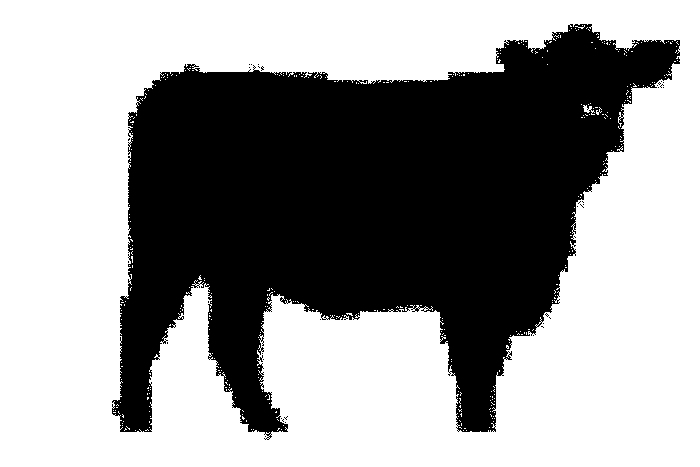
\includegraphics[width=\textwidth,height=\textheight,keepaspectratio]{process/cow-black-and-white.jpg}
  \end{figure}

  \item Denoising this black-and-white image: Although converting a raster image to black-and-white comes a long way for vectorizing that image, the black-and-white image after the conversion is in fact, noisy. That is, the image is in black-and-white and for the most part, represents the shape of the structure that is depicted in the original raster image. However, there is same granularity, some noise, on the edges of the structure after the conversion. This is, of course something that is not desirable, since this only makes it harder to trace this image. That is, tracing the image in this state can result in multiple, irrelevant curves in the output, instead of a single curve that represents the structure. This is not something we want, since the irrelevant curves will simply result in erroneous structure constructions. Hence, in order to remove this unwanted effect, we simply denoise the resulting black-and-white image and hence, we obtain a smooth black-and-white image that is much more suitable for producing a fine and sharp vector image.

  The image formed after this step is the following:

  \begin{figure}[H]
    \centering
    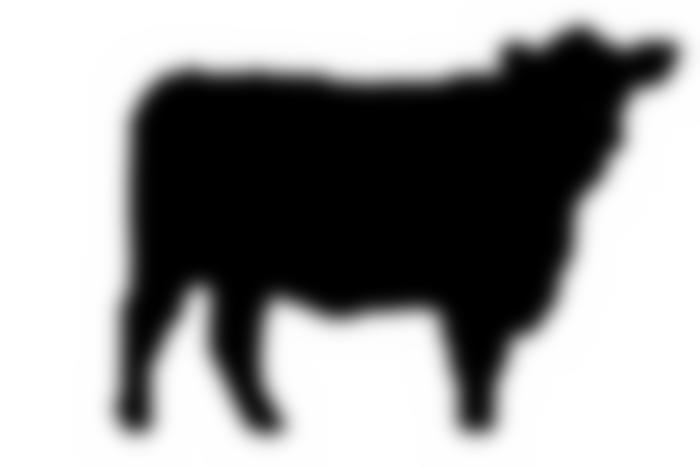
\includegraphics[width=\textwidth,height=\textheight,keepaspectratio]{process/cow-black-and-white-denoised.jpg}
  \end{figure}

  \item "Tracing" this denoised, black-and-white image in order to obtain an SVG image: Theoretically, the raster image can be traced into a vector image using any method. Specifically, we are using the open source program named Potrace, written by Peter Selinger, for this task.
  One of the rather important reasons for converting the original raster image to black-and-white, instead of directly tracing it (that is, creating a vector image out of it) is that the tracer (vectorizer) software that we use, Potrace, works only on black-and-white images. That is, the behavior of Potrace for non black-and-white images is undefined. Hence, we opt to use a black-and-white image as the input for Potrace. That is the main reason that we convert the original raster image into black-and-white, instead of feeding it to Potrace as is.

  The image formed after this step is the following:

  \begin{figure}[H]
    \centering
    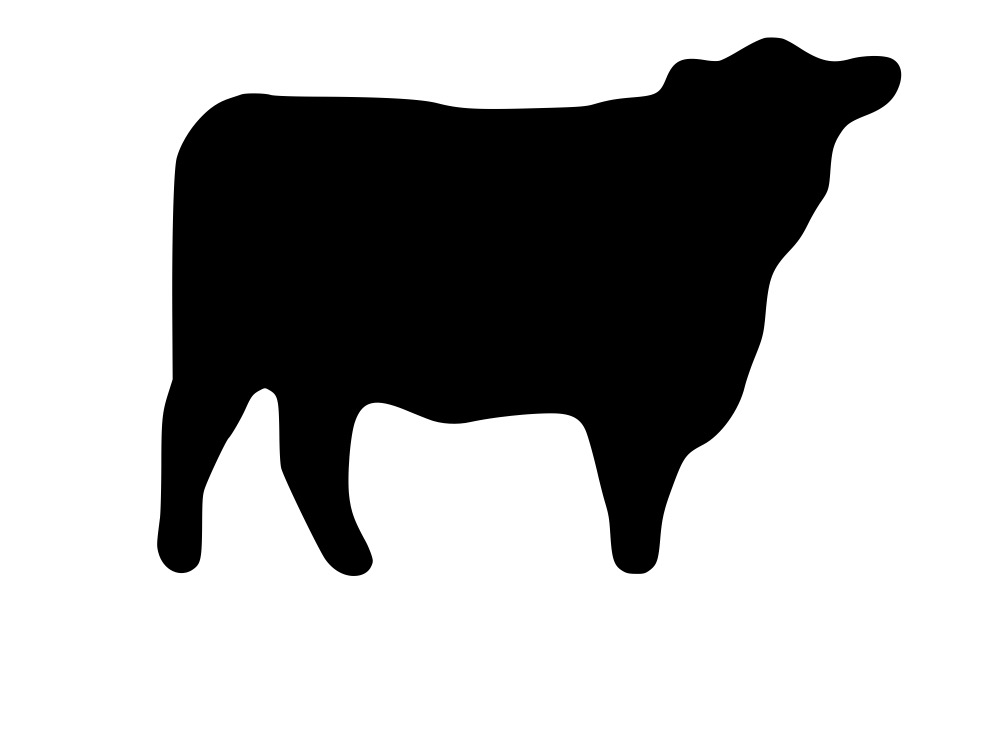
\includegraphics[width=\textwidth,height=\textheight,keepaspectratio]{process/cow-black-and-white-denoised-converted-from-svg.jpg}
  \end{figure}

  \item Potrace traces the raster image into a vector image successfully. However, in the output, it uses SVG \lstinline{path} elements. For general purposes, this is perfectly fine. However, the main reason that we need the SVG is in order to be able to cleanly determine the outlines of the structure represented by the raster image. The reason for doing this is as follows: When the image is in one of the raster formats, determining the outline of the structure represented by this raster image is not very straightforward. However, since all we need for the purpose of generating a Science Birds structure is the outline of the structure represented in the raster image, we need a way to attain the information about the outline of the structure represented in the raster image. This is where the SVG, specifically an SVG with a \lstinline{polygon} element, comes into play. Normally raster images represent an image as a collection of pixels. Basically, in a raster image, there is no notion of a shape. That is, in a raster image, mostly the image is represented as a collection of independent picture elements (pixels). Hence, in a raster image, it is not straightforward at all to determine what sort of shape is being represented by this image. In other words, there is no proper notion of a "shape" in a raster image.

  The image formed after this step is the following:

  \begin{figure}[H]
    \centering
    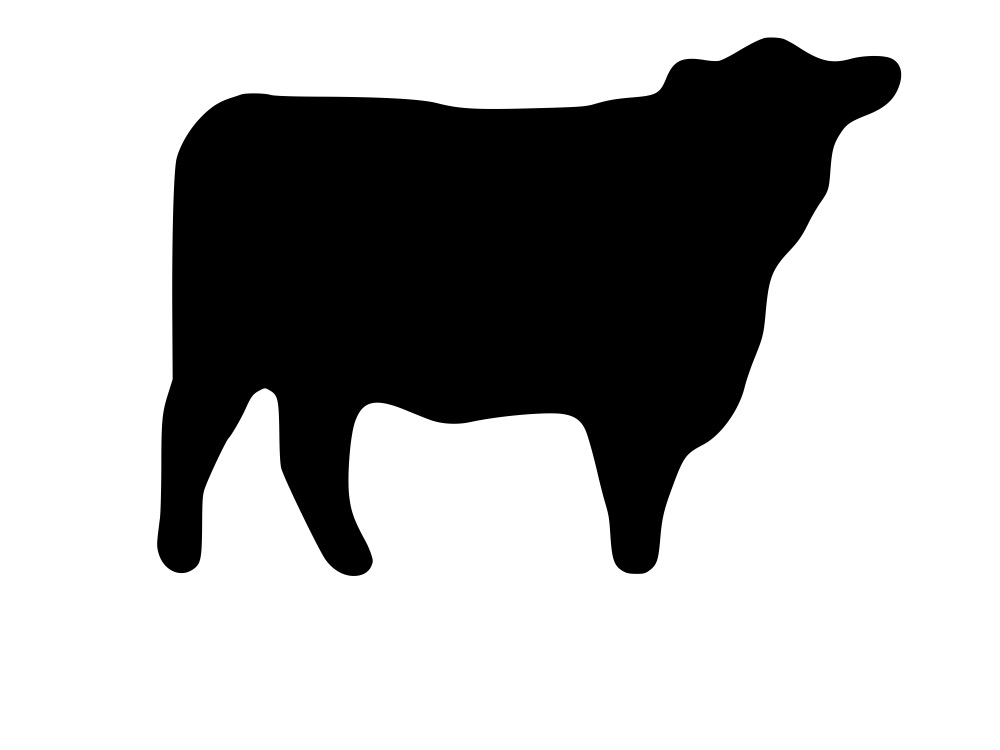
\includegraphics[width=\textwidth,height=\textheight,keepaspectratio]{process/cow-black-and-white-denoised-polygon.jpg}
  \end{figure}
\end{enumerate}

On the other hand, vector image formats are the opposite of raster image formats. While raster image formats usually represent an image as an unrelated collection of picture elements, a vector image format, on the other hand, represents an image as a collection of shapes. It is this fundamental difference in the approach of image representation that differentiates the raster and the vector image formats. Since a vector format represents an image as a collection of shapes, a vector image is not as prone to alterations in the image quality as a result of altering the viewing point of the image. For example, a vector image is almost immune to degradation in quality when zooming in the image. It simply shows the zoomed in detail of the image as represented among the shape declarations of the vector image. It is precisely this characteristic of vector images, specifically SVG, that catches our attention. As we have stated before, for the purpose of generating a Science Birds level from an input raster image, all the information that we need from that raster image is simply the shape, that is, the outline, that this raster image represents. This outline information is best conveyed the level generator with an SVG image that represents the image with an SVG \lstinline{polygon} element. Hence, this is precisely the reason that we need an SVG image with a \lstinline{polygon} element in order to cleanly attain the information about the outline of the structure represented in the raster image.

\chapter{Algorithm}

After obtaining the Scalable Vector Graphics (SVG) image which is produced by:

\begin{enumerate}
  \item Converting the raster image into black-and-white
  \item Denoising it
  \item Tracing it
\end{enumerate}

\noindent
we feed this SVG image into the main script. In the main script, the following happens:

\begin{enumerate}
  \item The configuration file is read in order to determine where should the output level file be written to. The output level file is an XML file which contains a description of a Science Birds level. Overall, it has the following structure:

  \begin{lstlisting}
  <?xml version="1.0" encoding="utf-8"?>
  <Level>
    <Camera x="" y="" minWidth="" maxWidth="">
    <Birds>
      <Bird type="" />
      ...
    </Birds>
    <Slingshot x="" y="" >
    <GameObjects>
      <Block type="" material="" x="" y="" rotation="" />
      ...
      <Pig type="" x="" y="" rotation=""/>
      ...
      <Platform type="" x="" y="" scaleX="" scaleY="" />
      ...
      <TNT type="" x="" y="" rotation="" />
      ...
    </GameObjects>
  </Level>
  \end{lstlisting}

  Note that Science Birds developers have opted not to be very strict about the validity of XML in the level files. That is, some elements in the level actually turn the XML into invalid XML. Nevertheless, the level is still openable and it is still playable. Some examples to these invalid elements would be the elements \lstinline{Camera} and \lstinline{Slingshot}. Although these elements do not have a separate closing element, they don't end with \lstinline{/>} as they should be in valid XML. Instead, they end with \lstinline{>}, just like a self-closing tag in HTML. However, precisely speaking, a Science Birds level file is not an HTML file, it is an XML file. Hence, the aforementioned non-conforming elements should have either:

  \begin{enumerate}
    \item Had a closing tag.

    or

    \item Ended the single tag elements with \lstinline{>}, instead of \lstinline{/>}.
  \end{enumerate}

  in order to ensure that the XML files of Sciene Birds levels are, indeed, valid XML files.

  The sample level file structure scheme above demonstrates what a generic level would be similar to. However, it doesn't go into detail of explaining what these elements are, what is their use or how do their attributes alter or enhance their behavior. In order to gain a solid understanding of the level scheme of Science Birds, we need to understand the individual elements, and the attributes of each of these individual elements that make up a Science Birds level. To do so, we need to examine the sample Science Birds XML level structure step-by-step, examining one line at each step:

  \begin{enumerate}
    \item

    \begin{lstlisting}
      <?xml version="1.0" encoding="utf-8"?>
    \end{lstlisting}

    This is simply a generic XML file declaration. Without this element, we wouldn't be able to claim that a Science Birds level file is indeed, an XML file, even though it might be composed of elements within angular brackets and the file extension in a Science Birds level filename is \lstinline{.xml}.

    \item

    \begin{lstlisting}
      <Level>
    \end{lstlisting}

    This is the top-level container element that contains all the other elements that are necessary to be able to construct a complete, working Science Birds level. This is actually a container element. It is the only top-level element apart from the XML declaration line.

    \item

    \begin{lstlisting}
      <Camera>
    \end{lstlisting}

    This element exists to describe where should be the view be when the level starts, and what how large should it be.

    \item

    \begin{lstlisting}
      <Birds>
    \end{lstlisting}

    This is the element that contains all \lstinline{<Bird>} elements. In other words, this is a container element for the \lstinline{<Bird>} elements.

    \item

    \begin{lstlisting}
      <Bird>
    \end{lstlisting}

    This is the element that adds a bird to the list of birds that can be used in this level. There are different types of birds. These types are:

    \begin{enumerate}
      \item BirdWhite

      BirdWhite is a bird that is comparatively larger than the rest of the birds. The large size of this bird gives the advantage of being able to knock down more blocks due to:

      \begin{enumerate}
        \item Larger impact area.
        \item Higher impact force due to higher momentum.
      \end{enumerate}

      \begin{figure}[H]
        
\includegraphics[width=.5\textwidth,keepaspectratio]{birds/white.png}
      \end{figure}

      \item BirdBlue

      BirdBlue is a regular bird that is smaller than BirdWhite.

      \begin{figure}[H]
        
\includegraphics[width=.5\textwidth,keepaspectratio]{birds/blue.png}
      \end{figure}

      \item BirdYellow

      BirdYellow is around the same size with BirdBlue, only that it is of yellow color.

      \begin{figure}[H]
        
\includegraphics[width=.5\textwidth,keepaspectratio]{birds/yellow.png}
      \end{figure}

      \item BirdRed

      BirdRed is similar to BirdBlue and BirdYellow, only that it is of red color.

      \begin{figure}[H]
        
\includegraphics[width=.5\textwidth,keepaspectratio]{birds/red.png}
      \end{figure}

      \item BirdBlack

      BirdBlack is very similar to BirdWhite in terms of size. However, BirdBlack has one property that is not observed in any of the other birds. It has the ability to explode. Upon making the first contact with any kind of surface, be it the ground, a block, a platform, a pig or a TNT block, BirdBlack becomes "rigged to explode". This "rigged to explode" state is expressed by the BirdBlack's body flashing red intermittently. That is, it's body is covered with a red hue, and then it becomes normal. This state repeats a couple times a second until the bird explodes, which takes a couple seconds. Upon explosion, any movable thing that is in the immediate surrounding of the BirdBlack is pushed away from BirdBlack. This can help with knocking down more blocks and eliminating more pigs (that is, enemies), if the BirdBlack is launched in a manner that the explosion will happen in a strategically beneficial place which will allow these.

      \begin{figure}[H]
        
\includegraphics[width=.5\textwidth,keepaspectratio]{birds/black.png}
      \end{figure}
    \end{enumerate}

    \item

    \begin{lstlisting}
      <Slingshot>
    \end{lstlisting}

    The slingshot is used to launch the birds into a trajectory in order to knock down the structures and to eliminate the enemies that are present on the level. Its attributes \lstinline{x} and \lstinline{y} are used to express the location on the two-dimensional level platform that the slingshot should be placed to.

    \item

    \begin{lstlisting}
      <GameObjects>
    \end{lstlisting}

    This is a container element that is used to contain every single element in a Science Birds level, apart from the birds and the slingshot. That is, this element is used to contain all elements that a bird is able to make contact with, with of without effect. Specifically, it can contain \lstinline{<Block>}, \lstinline{<Platform>}, \lstinline{<Pig>} and \lstinline{<TNT>} elements.

    \item

    \begin{lstlisting}
      <Block>
    \end{lstlisting}

    This is the main element that is used to construct structures. Basically, a Science Birds structure is an aggregation of \lstinline{<Block>} elements. Technically, \lstinline{<Platform>} elements and \lstinline{<TNT>} elements can be used as part of a structure as well, along with using a \lstinline{<Pig>} element as the enemy. However, in this programmatic content generator, a Science Birds structure consists only of \lstinline{<Block>} elements.

    There are precisely thirteen different shapes of blocks. Each block type has four integrity conditions. That is, when the blocks hadn't taken any damage, they are in perfect condition. As they take more damage, their condition changes. Finally, after enough damage, a block disappears and the player gets points from this.

    Of the thirteen types of blocks, twelve of them has variations in all three materials, namely "ice", "wood" and "stone". Only one of them can be drawn in only one material, which is Ice Square.

    Each of the four different integrity conditions of the blocks are represented by a different sprite for each block type. Hence, the total number of sprites for all blocks is as follows:

        12 * 3 * 4 + 4 = 148

    The blocks, except the single material type block Ice Square, are the following:

    \begin{itemize}
      \item Small Circle
      \item Circle
      \item Triangle
      \item Triangle with Hole
      \item Small Square
      \item Square
      \item Square with Hole
      \item Tiny Rectangle
      \item Small Rectangle
      \item Medium Rectangle
      \item Big Rectangle
      \item Fat Rectangle
    \end{itemize}

    So, the first two attributes of the \lstinline{<Block>} element are now clear. The \lstinline{type} attribute is used to indicate which block type this block should stand for, where those block types are listed above. On the other hand, the \lstinline{material} attribute is used to specify which material this block should be of. The possible materials are:

    \begin{itemize}
      \item Ice
      \item Wood
      \item Stone
    \end{itemize}

    The remaining attributes are \lstinline{x}, \lstinline{y} and \lstinline{rotation}. These have the following respective purposes:

    x: This attribute specifies the location of this block on the X coordinate. The origin is the top-left location and the X coordinate increases towards right.

    y: This attribute specifies the location of this block on the Y coordinate. The origin is the top-left location and the Y coordinate increases towards down.

    rotation: This attribute specifies the angle which this block is placed according to.

    \item

    \begin{lstlisting}
      <Pig>
    \end{lstlisting}

    This element specifies a pig. The attributes are as follows:

    \begin{itemize}
      \item type: This attribute specifies the type of the pig. Possible values are:

      \begin{itemize}
        \item BasicBig
        \item BasicMedium
        \item BasicSmall
      \end{itemize}

      \item x: This attribute specifies the location of this pig on the X coordinate.
      \item y: This attribute specifies the location of this pig on the Y coordinate.
      rotation: This attribute specifies the angle which this pig is placed according to.
    \end{itemize}

    \item

    \begin{lstlisting}
      <TNT>
    \end{lstlisting}

    This element represents a TNT block. A TNT block is a block that is rigged to blow. Upon activation, a countdown for that TNT block starts and at the end of the countdown, the TNT block explodes. A TNT block becomes activated whenever another block hits it. The explosion of a TNT block destroys blocks and eliminates enemies in the surrounding of the TNT block, within a certain diameter.
  \end{enumerate}

  \item After the configuration file has been read, the following parameters are extracted from it:

  \begin{enumerate}
    \item LevelPath: This parameter specifies the directory where the Science Birds levels should be written to, in order to be able to play them upon launching Science Birds.

    \item PrimaryBlock: This parameter specifies the block that is used to construct the structure. A structure in Science Birds Programmatic Content Generator is constructed using two types of blocks: primary block and platform block. primary block is the block that is structure is initially constructed from. That is, the structure initially solely consists of primary blocks.

    \item PlatformBlock: This parameter specifies the block that is used to support the primary blocks that have nothing under them to prevent them from falling. After the structure is initially constructed solely by using primary blocks, in most cases, there are some primary blocks that happens to have nothing under them. Had these blocks be left in this state, they would simply start free falling upon level start. This is, of course, not a desirable thing, since in such case, the player would get undeserved points due to elimination of some blocks because of free falling. Also, the free falling blocks might result in imbalances in the structure and hence, result in toppling of the structure as well. Because of these reasons, in order to have a level with a stable and playable structure, we must make sure that there shouldn't be any blocks without anything supporting them below. Hence, the program determines where exactly to place these platforms and places these platform blocks accordingly. The details of the platform insertion procedure is examined in detail in the latter parts of this dissertation.

    \item NumberOfPrimaryBlocksOnXAxis: This parameter specifies how many primary blocks should be placed to X axis. Initially, one might think that this should be determined by dividing the width of the structure to the width of the primary block. This is, in general, an accurate and sensible approach. However, there is a caveat: If the structure too wide, and the primary block's width is not wide enough, there will be a lot of blocks on the X axis, and as a result of this, on the Y axis as well. Hence, the structure will be composed of too many blocks. Similarly, if the structure is rather thin, and the primary block's width is wide relative to the width of the primary block, there will be too few blocks on the X axis, and as a result of this, on the Y axis as well. Hence, the structure will be composed of too few blocks.
  \end{enumerate}

  Neither of these situations desirable. If the structure happens to be constructed of too many blocks, there will be three problems:

  \begin{enumerate}
    \item The rendering of these blocks will take more resources and hence, it might lead to a degraded experience.

    \item Since there will be too many blocks, it will take more effort to knock down the structure. Similarly for eliminating all the pigs in the level. For example, it might require more birds to knock down the structure or eliminate all the pigs. In most cases, this is something that degrades the experience. Hence, having more than necessary amount of blocks for a structure is something to be best avoided.
  \end{enumerate}

  In the same fashion, having too few blocks in a structure is an undesirable thing as well. If the structure is composed of too few blocks, it most likely will be too thin and short. In such case, most likely there won't be enough space in the structure to insert platforms and place pigs (enemies). There cannot be a playable level without any pigs, since the goal of each level is to eliminate every single pig in that level. For these reasons, having a level with a too thin structure is not something that we would like either.

  So, we understood that if we decide on the number of primary blocks on the X axis by dividing the width of the structure to the width of the primary block, there is room for numerous problems. Hence, dividing the width of the structure to the width of the primary block is not the optimal method to decide on the number of primary blocks on the X axis and implicitly, the number of blocks of the whole structure.

  \begin{figure}[h]
    \centering
    \caption{A structure with inadequate number of blocks for pig insertion}
    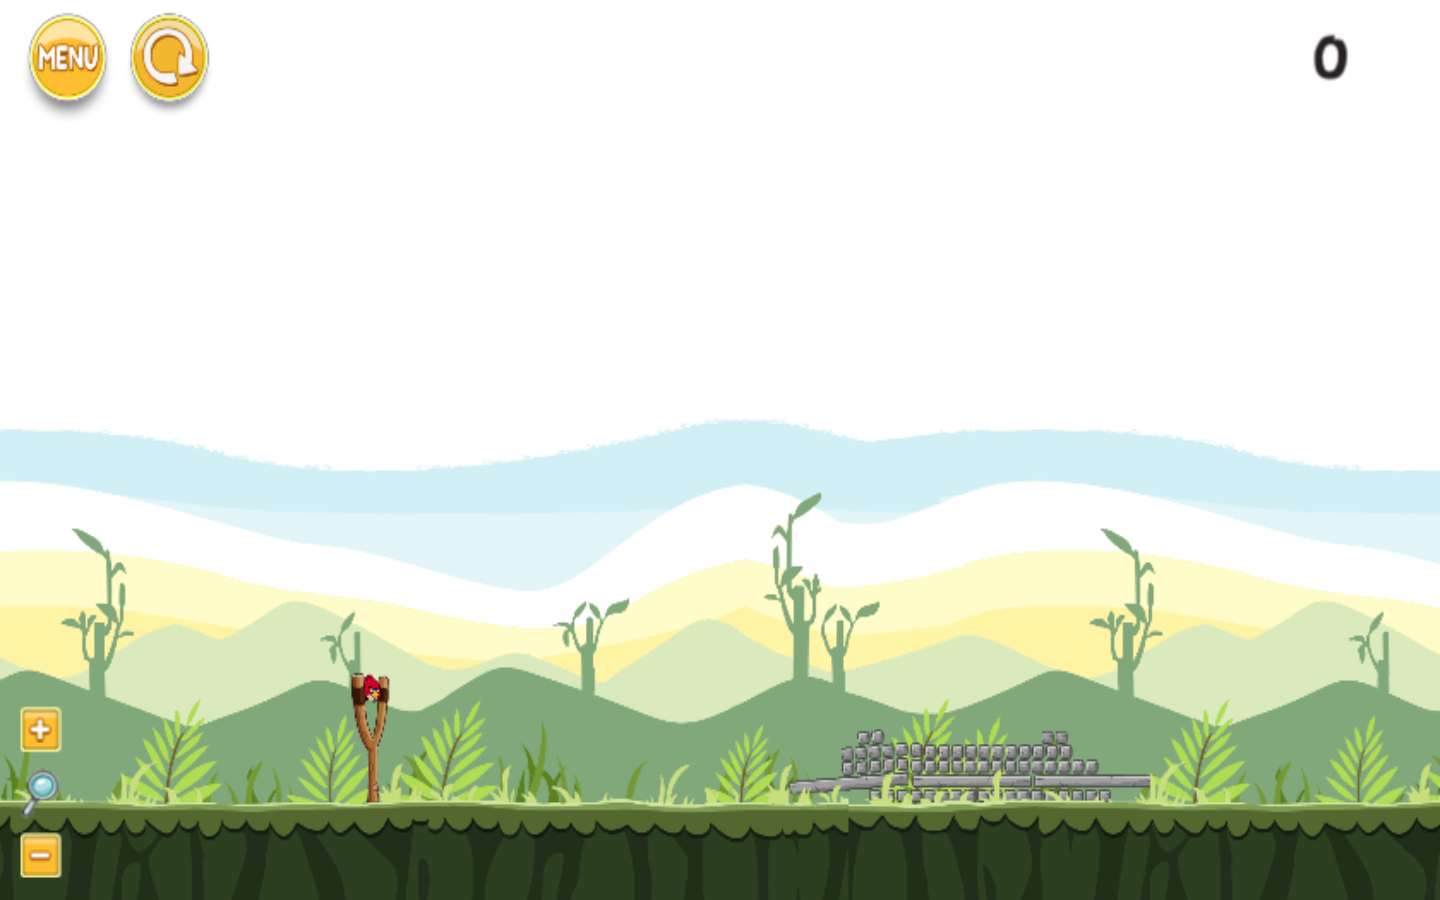
\includegraphics[width=\textwidth,height=\textheight,keepaspectratio]{process/inadequete_number_of_blocks.png}
  \end{figure}

  What then, might be a better way to decide on the number of primary blocks on the X axis? As it is currently implemented, deciding on it manually, that is, using a parameter seems to be the best way now. One point to clarify here is that if we decide on the number of primary blocks on the X axis manually, instead of dividing the width of the structure to the width of the primary block, then how are we going to decide on the number of primary blocks on the Y axis? Should we use another parameter for that as well? Well, the answer is no, because doing that would simply remove the dependence between the structure's width of the X axis and on the Y axis. Removing this would result in the created structure being out of shape. Hence, in order not to cause such an issue, we instead proportionate the dimensions of the primary block to the dimensions required by the specified number of primary blocks on the X axis. Precisely, we do this as follows:

  \begin{enumerate}
    \item Divide the width of the structure to the specified number of primary blocks on the X axis.

    \item Divide this result to the actual width of the primary block. The result of this gives us the block factor.

    \item Multiply the block factor with the height of the primary block.

    \item Divide the structure height by the result of the calculation done at step 3. The result will give the number of blocks that should be on the Y axis.
  \end{enumerate}

  \item After reading the arguments, we read the SVG file in order to determine the shape and boundaries of the structure that we are about to construct. This is done as follows:

  \begin{enumerate}
    \item Read the SVG file.
    \item Find the SVG \lstinline{<polygon>} element in it.
    \item Get the list of points in that \lstinline{<polygon>} element.
    \item Using this list of points, construct a \lstinline{Polygon} object. This is done with the help of a library called Shapely.
    \item Rotate this polygon object 180 degrees (upside-down). The reason for this step is that Potrace generates the SVG image in an upside-down form. In order to properly use the image to construct a Science Birds structure, we need to access the SVG image's proper (upright) version.
  \end{enumerate}

  \item After reading the SVG file and constructing a polygon from it, we initialize a Structure object. A structure object is an object that represents a Science Birds structure. It represents every aspect of it. Some of these are:

  \begin{enumerate}
    \item The original polygon shape that is read from the SVG file.
    \item All of the arguments:
    \begin{enumerate}
      \item The level path.
      \item The primary block type.
      \item The platform block type.
      \item Number of primary blocks on X axis.
    \end{enumerate}
    \item Number of primary blocks required to cover pig width: In this PCG, the pigs are placed by removing some primary blocks and placing the pig to the bottom center of the cavity as a result of this removal. Hence, the width created by removing the primary blocks should be at least as long as the pig's width. Otherwise, the pig simply wouldn't fit in the cavity created by removing the pigs. Hence, in order to determine this width, we make a calculation to determine the number of primary blocks to remove, so that the width created by this removal will at be at least equal to the width of a pig.
    \item Number of primary blocks required to cover pig height: This is the same concept as "number of primary blocks required to cover pig width".
    \item Primary block factor: This is the concept that we have mentioned about in the definition of "NumberOfPrimaryBlocksOnXAxis" parameter. To remember what we have stated there, the primary block factor is a ratio that dictates the factor the primary block dimensions need to be multiplied with in order to cover the structure width and the structure height. Note that the structure width and the structure height simply refers to the width and height of the rectangle that would contain the structure that is expressed in the SVG file. In other words, the "width" and "height" refer to the containing rectangle of the structure that is expressed in the SVG file.
    \item Factored primary block width: This is the distance that is calculated by multiplying the primary block width with the primary block factor.
    \item Factored primary block height: This is the distance that is calculated by multiplying the primary block height with the primary block factor.
    \item Number of primary blocks on X axis: This is calculated by dividing the structure width by the factored primary block width.
    \item Number of primary blocks on Y axis: This is calculated by dividing the structure height by the factored primary block height.
    \item Original blocks: This is the matrix (list of lists) that holds the blocks of the structure location by location. As you can realize, this is not something that has been passed to the Structure class' constructor. That means this must be computed within the Structure class. Precisely, this is done in the \lstinline{get_blocks} method of the Structure class. The algorithm is basically as follows:

    \begin{enumerate}
      \item The structure shape that is obtained from the input SVG is partitioned into tiles, where the length and width of the tiles are dictated by the parameters \lstinline{num_primary_blocks_on_x_axis} and \lstinline{num_primary_blocks_on_y_axis}.
      \item Each tile is composed of:

      \begin{enumerate}
        \item Either only by a structure.
        \item Or only by void.
        \item Or both some structure and some void.
      \end{enumerate}

      If the area of the structure within that tile is greater than or equal to half of the area of a tile, we decide that there should be a primary block inserted for this location. Otherwise, we leave this tile empty.

      We repeat this procedure for each tile and in the end, we obtain a list of lists, that contains True or False values, indicating that there should be a block in that location or not.
    \end{enumerate}

    \item Blocks: This parameter is very similar to original blocks parameter, with the only difference being that this is the version of original blocks that is transposed and inverted. The original blocks parameter starts from top-left and continues towards bottom-right, as this is the natural procession order in SVG (and most image formats). However, for the purposes of constructing a Science Birds structure out of a matrix of blocks, the most practical way is to start from bottom-left and go towards top-right. The reason is starting from the ground and building a column, then proceeding to the next column and building it, until all columns have been finished.

    \item Platforms: The platforms are obtained with the following algorithm:

    \begin{enumerate}
      \item Determine every block which has nothing underneath it.
      \item Determine the row number of each such block and add this row number to a set which contains the row indices for platforms to be inserted under.
      \item Repeat this for every block on the structure.
    \end{enumerate}

    These steps are for determining the necessary platforms. That is, they are for determining the rows to place platforms which are necessary in order to prevent blocks without anything under to free fall upon level start. In addition to the necessary platforms, there are also extra platforms. Extra platforms are the platforms inserted to the structure not because of preventing blocks from free falling, but to create places to be able to insert more pigs. The algorithm to insert extra platforms is as follows:

    \begin{enumerate}
      \item Determine the topmost and bottommost platform.
      \item Starting from the topmost platform and going above, insert an extra platform every Nth row, where N is equal to the number of primary blocks required to cover pig height.
      \item Similar to the previous step, starting from the bottommost platform and going below, insert an extra platform every Nth row, where N is equal to the number of primary blocks required to cover pig height.
    \end{enumerate}

    \item Platform blocks: In the previous step, we have determined the row indices where the platforms should be placed under. However, we still don't have the information about which lateral distance each platform block should be centered at. This is something that needs to be calculated. The reason is that although the primary blocks have fixed places, the platform blocks have not. That is, unlike the primary blocks, the platform blocks have lateral distances that can vary for each platform. Hence, the lateral distance of each platform block needs to be calculated individually.

    The reason for this is the following: Platform blocks are placed according to the placement of the primary blocks which the platform is located under. That is, the main reason for placing platform blocks is to support the primary blocks that have nothing underneath them. That is, the main reason is to prevent primary blocks without anything underneath them from free falling. Because of this, if a row is not filled with primary blocks, that is, if the primary blocks in a row does not start at the left edge of the shape's containing rectangle, and end at the end at the right edge of the shape's containing rectangle, then the distances of the platform blocks under that row is not regular, and they need to be custom calculated. The reason is that in such scenario, the platform blocks start and somewhere in the middle of the row, and end at somewhere in the middle of the row, instead of starting at the beginning and ending at the beginning. The algorithm to calculate the platform block locations is as follows:

    \begin{enumerate}
      \item Determine the leftmost primary block in the row which the platform is going to be placed under. We do this by determining the column index of the leftmost primary block in the row which the platform is going to be placed under.

      \item Determine the rightmost primary block in the row which the platform is going to be placed under. We do this by determining the column index of the rightmost primary block in the row which the platform is going to be placed under.

      \item Using the leftmost primary block index, rightmost primary block index, and the total number possible primary blocks in a row (which is obtained using the parameter named "number of primary blocks on X axis"), determine how many primary blocks there are between the leftmost primary block in the row and the rightmost primary block in the row.

      \item Using the number of blocks between the leftmost primary block in the row and the rightmost primary block in the row and using the width of the platform block, calculate the number of platform blocks required to cover the distance under the number of blocks between the leftmost primary block in the row and the rightmost primary block in the row, using platform blocks. This will give us the number of platform blocks required for that row.

      \item Using the number of blocks between the leftmost primary block in the row and the rightmost primary block in the row, compute the center of the region between the leftmost primary block in the row and the rightmost primary block in the row.

      \item Starting from the center of the region between the leftmost primary block in the row and the rightmost primary block in the row, we start inserting platform blocks. Platform blocks are inserted in a continuous manner. That is, except the initial iteration, at each iteration two platform blocks are added to the left and right ends of the current state of the platform. At the initial iteration, either one or two platform blocks are inserted. If the calculated number of platform blocks are odd, one platform block is inserted right at the center of the distance between the leftmost primary block in the row and the rightmost primary block in the row. This platform block is inserted in a manner such that the center of that platform block will correspond to the center of this distance.
    \end{enumerate}

    If, on the other hand, the calculated number of platform blocks are even, then there will be two blocks inserted at the initial iteration. The blocks will be inserted in such manner that the rightmost edge of the left platform block, and the leftmost edge of the right platform block will correspond to the center of the distance between the leftmost primary block in the row and the rightmost primary block in the row. The rest of the iterations are the same, two platform blocks are inserted at each iteration, one prepended to the left edge of the current platform, and the other appended to the right edge of the current platform.
  \end{enumerate}

  \item Pig indices: Pigs are inserted under every single platform block, where the previous platform is at least "number of primary blocks required to cover pig height" rows below the platform that contains this platform block. The reason is straightforward: If the previous platform is not at least "number of primary blocks required to cover pig height", then the pig won't have enough vertical space to fit in. This will cause the structure to have imbalances and to knock over.

  Another thing to note is that every pig is represented by only a single block index. That is, every pig is represented by the primary block's location that is at the center of the platform block that the pig is located under. Then, using this index, the pig is inserted to the center of this gap that is created by removing the blocks. The precise steps followed for block removal and pig insertion are as follows:

  \begin{enumerate}
    \item After a platform block is determined to be suitable for inserting a pig under, the index of the primary block that is right under and at the center of this platform block is determined. Index is the top-center location of the pig to be inserted.

    \item This block is removed.

    \item If the "number of primary blocks required to cover pig width" variable is greater than one, then additional blocks need to be removed as well. Removal of additional blocks are performed as follows:

    \begin{enumerate}
      \item Starting with the block that is at the immediate right of the center block, start removing the blocks by alternating between the block that is near (after) the rightmost edge of the gaps, and at the leftmost edge of the gaps.

      \item Repeat this "number of primary blocks required to cover pig height" times, going one row down at each step.

      To give a concrete example, let's say that the "number of primary blocks required to cover pig width" is 5. Then, the index offsets of the primary blocks to be cleared are as follows:

      0, 1, -1, 2, -2

      The "index offset" refers to the block position that is relative to the index of the primary block that is right under and that corresponds to the center of a particular platform block.

      Of course, this block removal is repeated as many times as the "number of primary blocks required to cover pig height", starting from the row that is immediately under the platform block and going downward.
    \end{enumerate}

    \item After the block removal is completed, the pig is inserted. The exact location to insert the pig is calculated as follows:

    \begin{enumerate}
      \item If the "number of primary blocks required to cover pig width" is an odd number, then the horizontal distance to place the pig is equal to the horizontal distance of the center of the primary block that is located right below the center of the platform block that this pig is being inserted under. If the "number of primary blocks required to cover pig width" is an even number, then we add half of the primary block's width to this distance to find the horizontal distance to insert the pig to.

      \item The vertical distance is calculated as follows:

      \begin{enumerate}
        \item Divide the "number of primary blocks required to cover pig height" by two. The division will result in a quotient and a remainder. Of course, if the "number of primary blocks required to cover pig height" is even, the remainder would be zero.

        \item Subtract "quotient + 1" from the row index of the platform that contains the platform block which the pig is being placed under.

        \item Calculate the height of the primary block row that corresponds to the resulting row index.

        \item If the "number of primary blocks required to cover pig height" is an even number, subtract half of the primary block's height from this height.
      \end{enumerate}
    \end{enumerate}
  \end{enumerate}
\end{enumerate}

This concludes the members of the Structure class.

\chapter{Appendix - Level Screenshots}

In this section, some sample images and Science Birds levels that are generated from these images are presented.

\begin{figure}
  
\includegraphics[width=\textwidth,height=\textheight,keepaspectratio]{levels/pictures/animals/cat.jpg}
  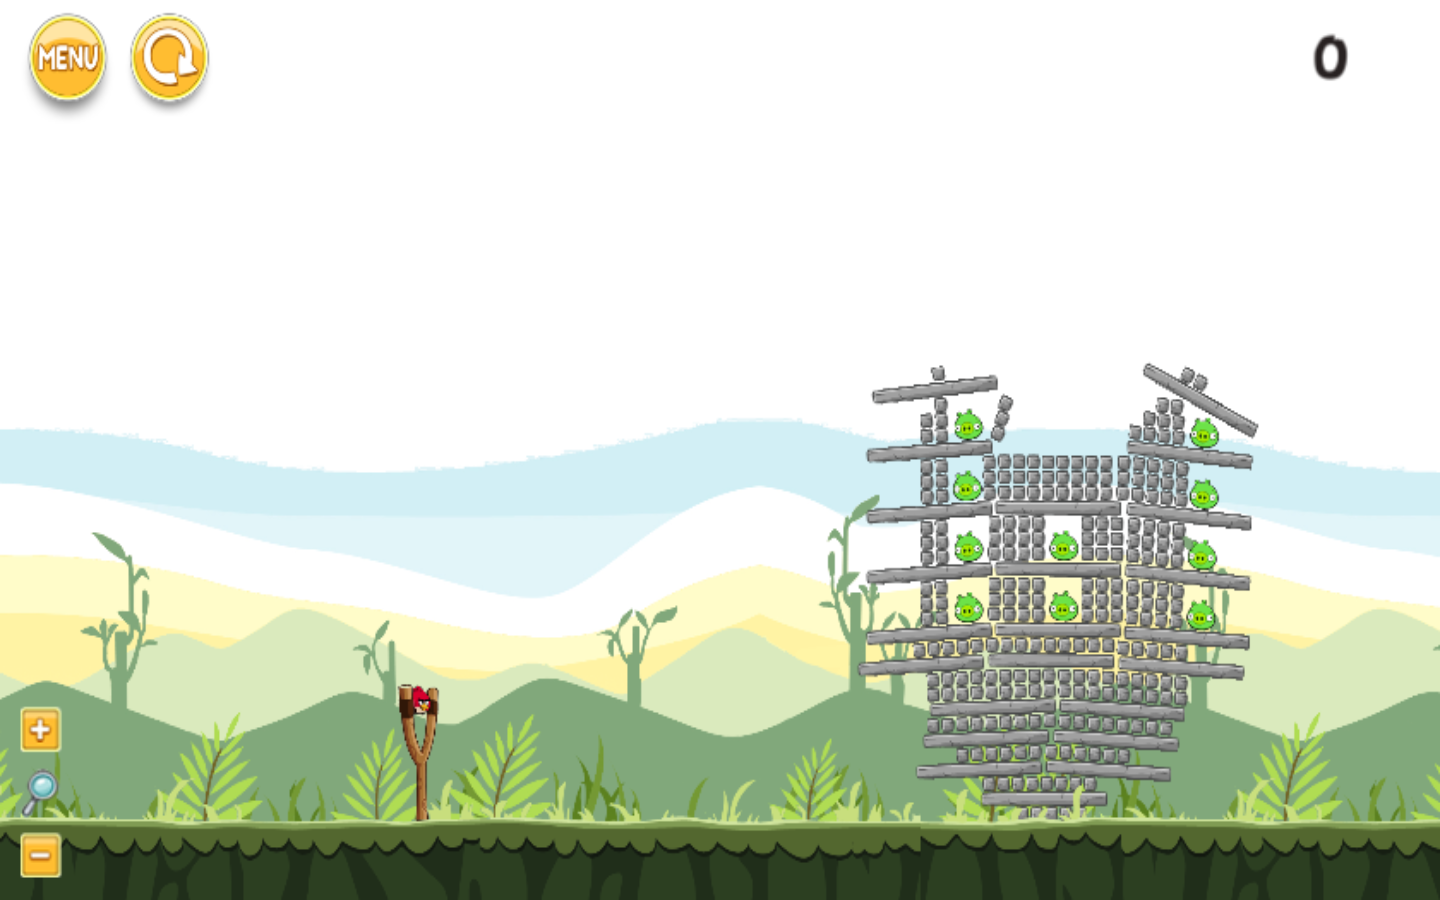
\includegraphics[width=\textwidth,height=\textheight,keepaspectratio]{levels/screenshots/animals/cat.png}
\end{figure}

\begin{figure}
  \includegraphics[width=\textwidth,height=\textheight,keepaspectratio]{levels/pictures/animals/cow.jpg}
  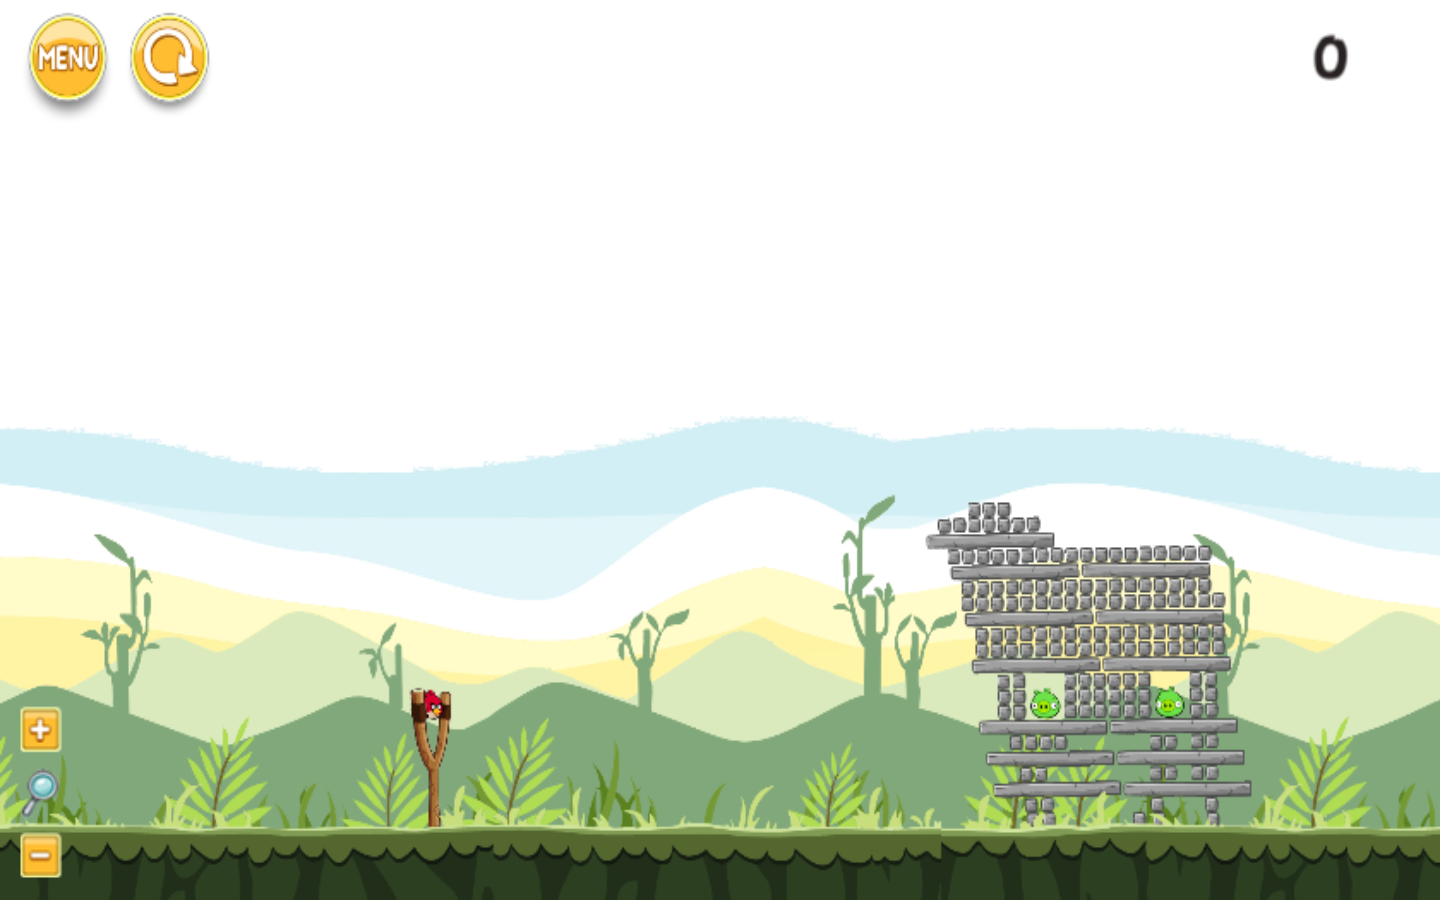
\includegraphics[width=\textwidth,height=\textheight,keepaspectratio]{levels/screenshots/animals/cow.png}
\end{figure}

\begin{figure}
  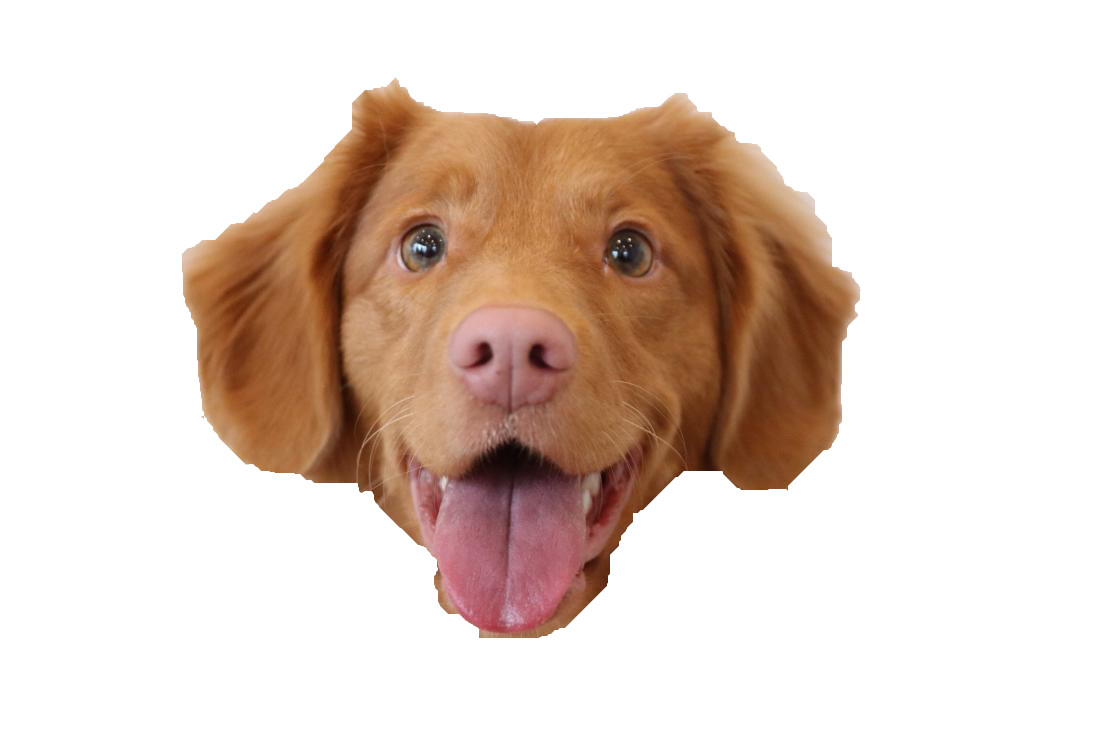
\includegraphics[width=\textwidth,height=\textheight,keepaspectratio]{levels/pictures/animals/dog.jpg}
  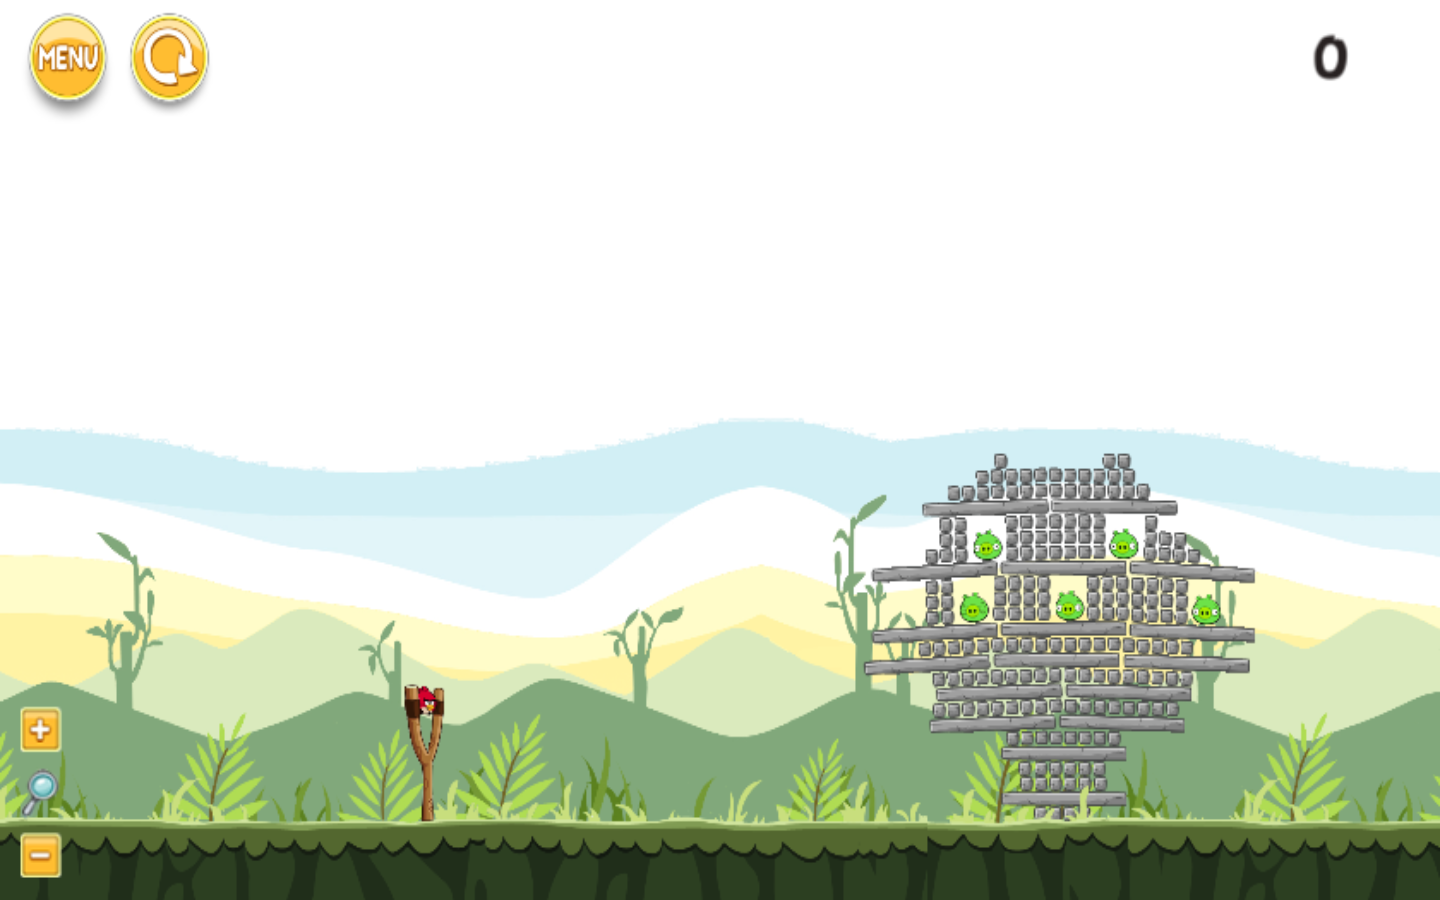
\includegraphics[width=\textwidth,height=\textheight,keepaspectratio]{levels/screenshots/animals/dog.png}
\end{figure}

\begin{figure}
  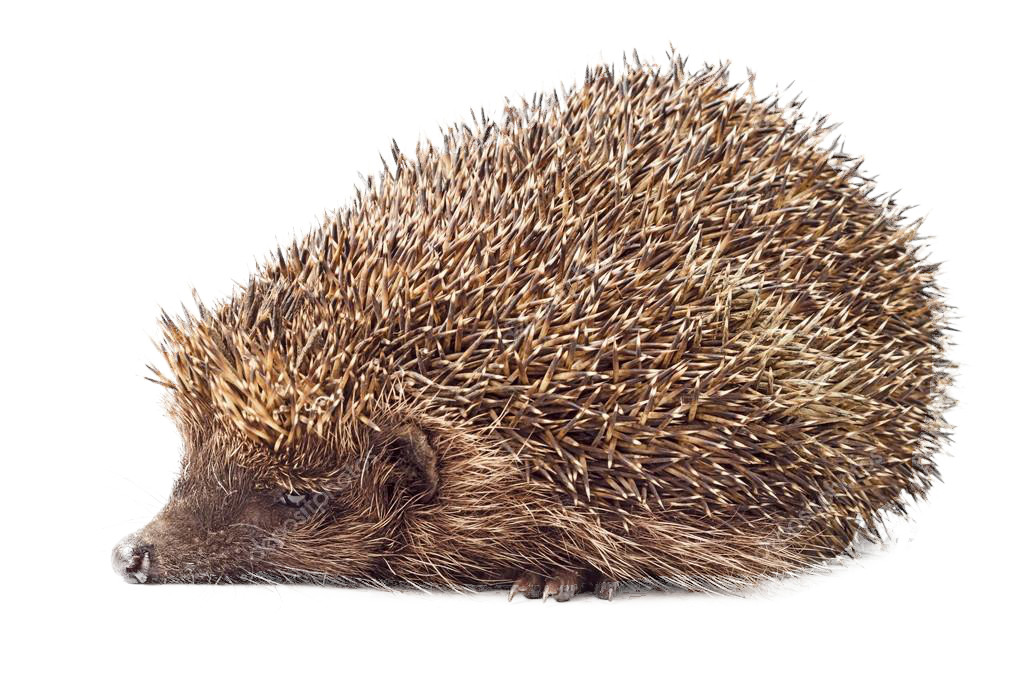
\includegraphics[width=\textwidth,height=\textheight,keepaspectratio]{levels/pictures/animals/hedgehog.jpg}
  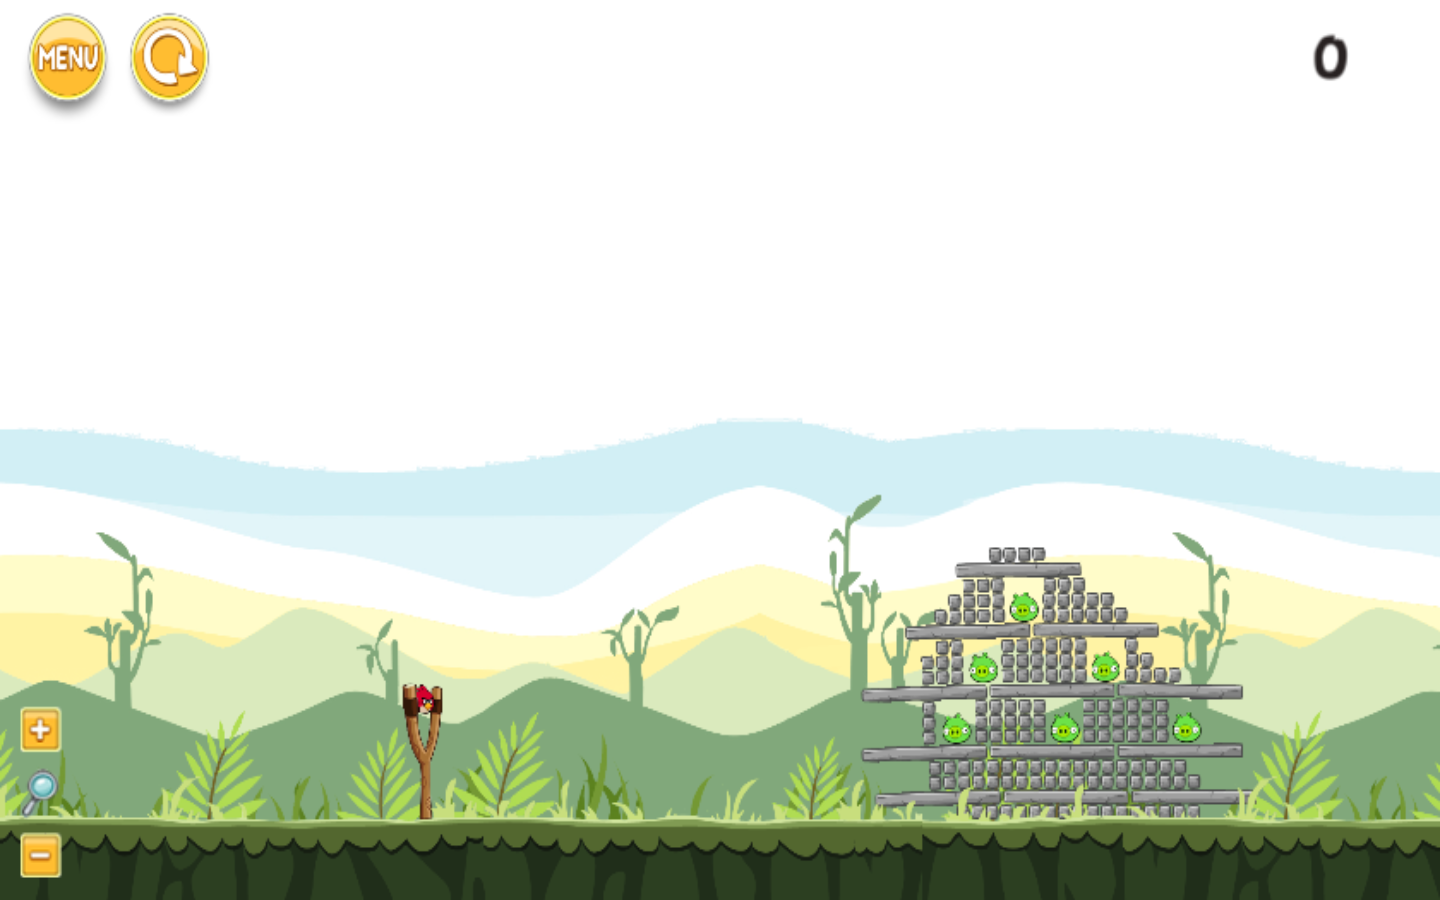
\includegraphics[width=\textwidth,height=\textheight,keepaspectratio]{levels/screenshots/animals/hedgehog.png}
\end{figure}

\begin{figure}
  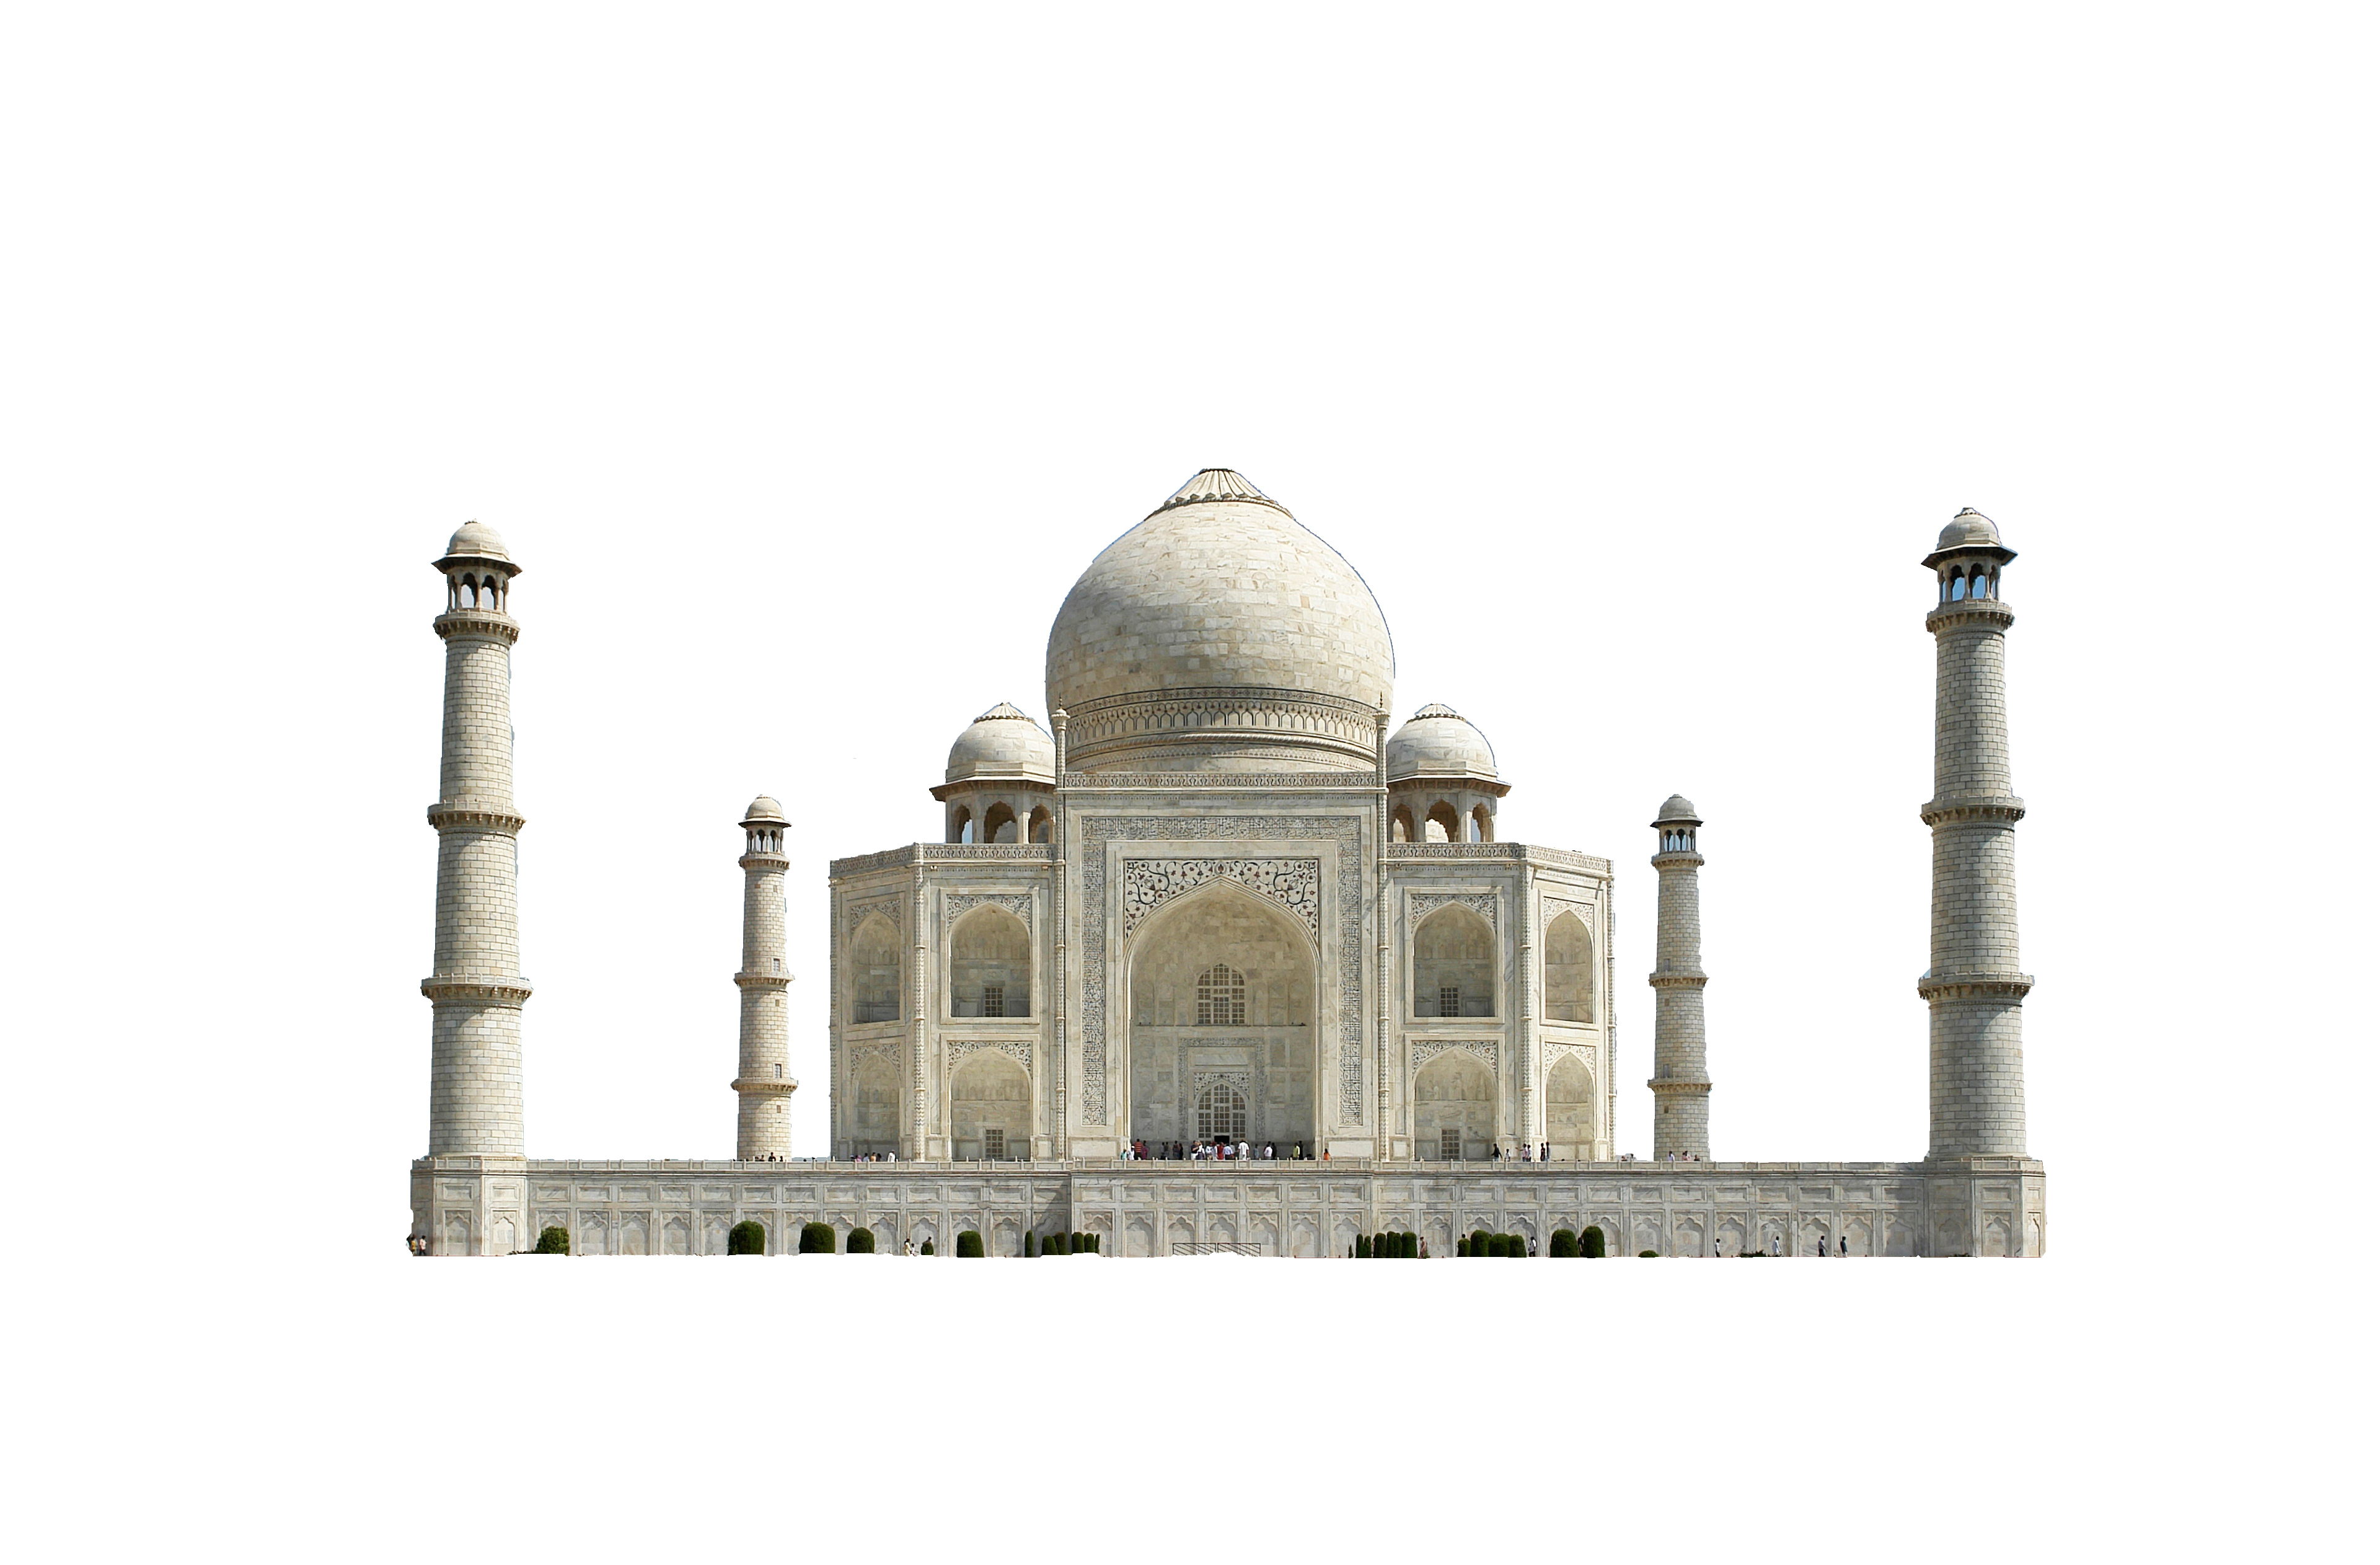
\includegraphics[width=\textwidth,height=\textheight,keepaspectratio]{levels/pictures/buildings/taj_mahal.jpg}
  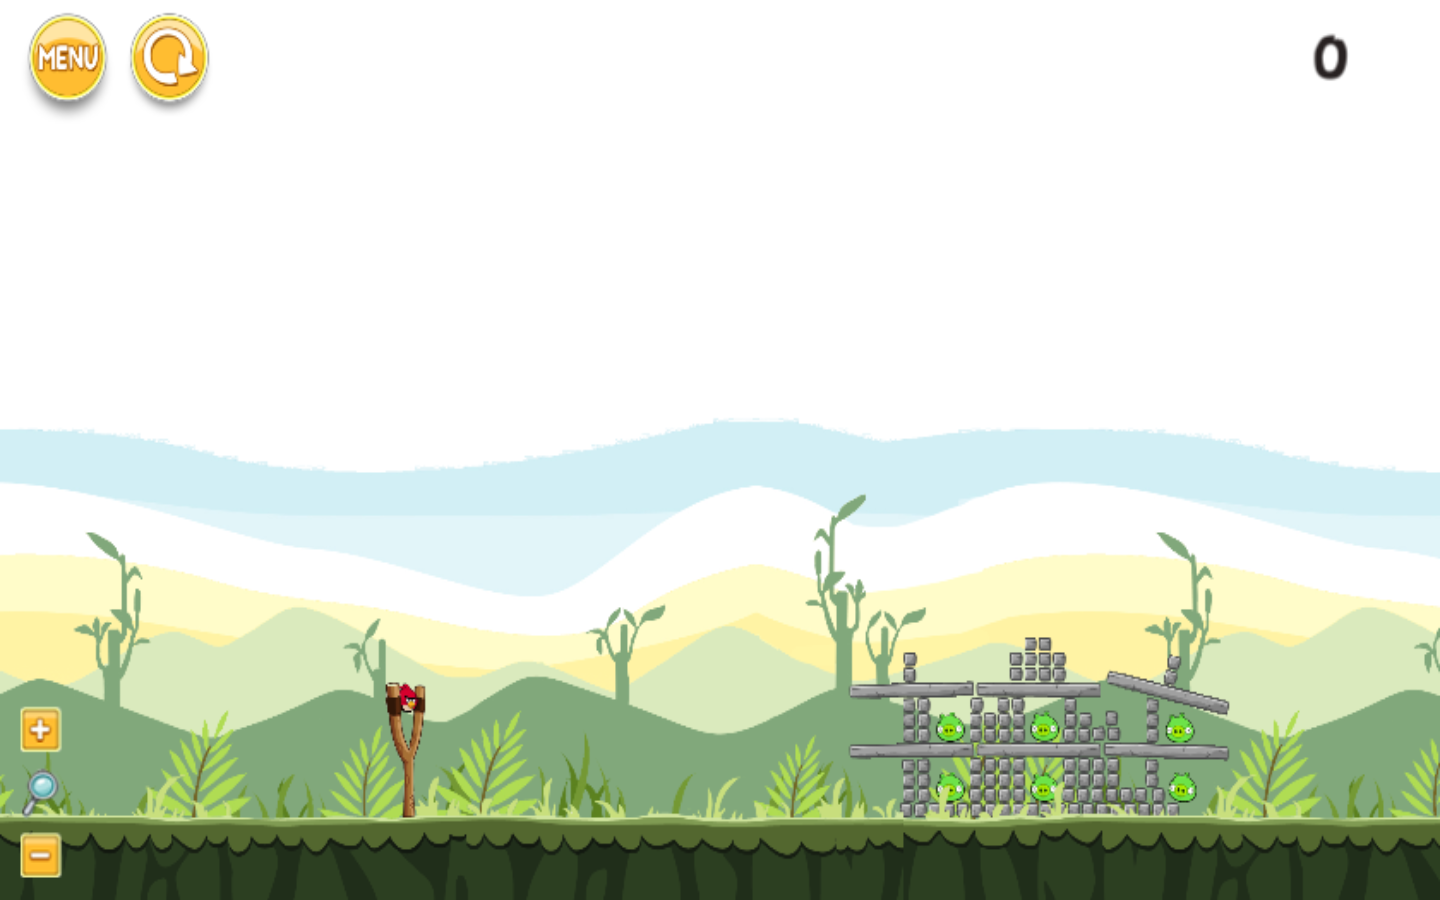
\includegraphics[width=\textwidth,height=\textheight,keepaspectratio]{levels/screenshots/buildings/taj_mahal.png}
\end{figure}

\begin{figure}
  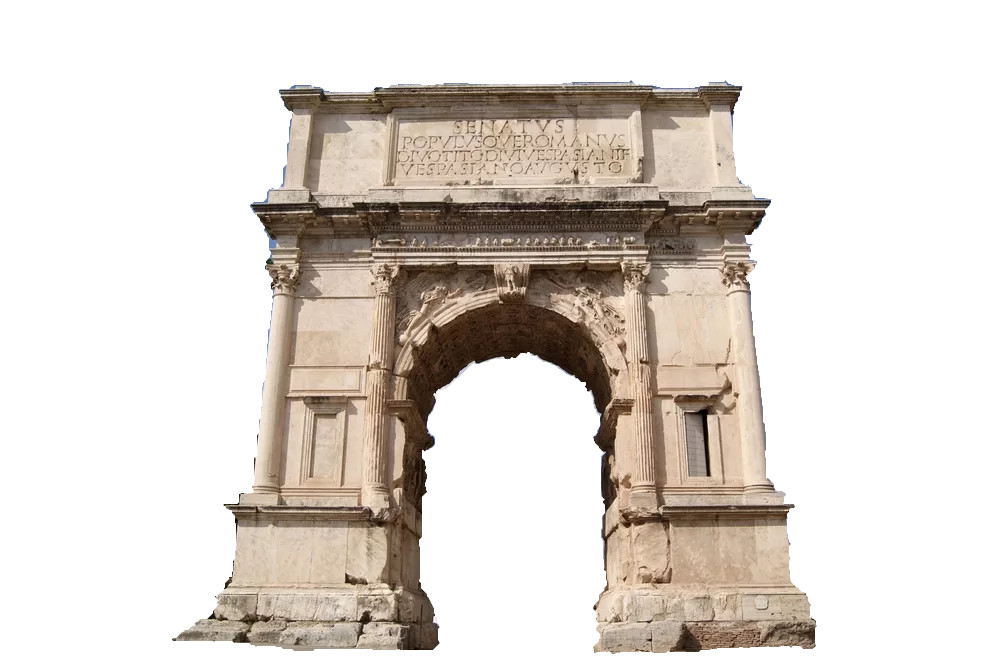
\includegraphics[width=\textwidth,height=\textheight,keepaspectratio]{levels/pictures/buildings/triumphal_arch.jpg}
  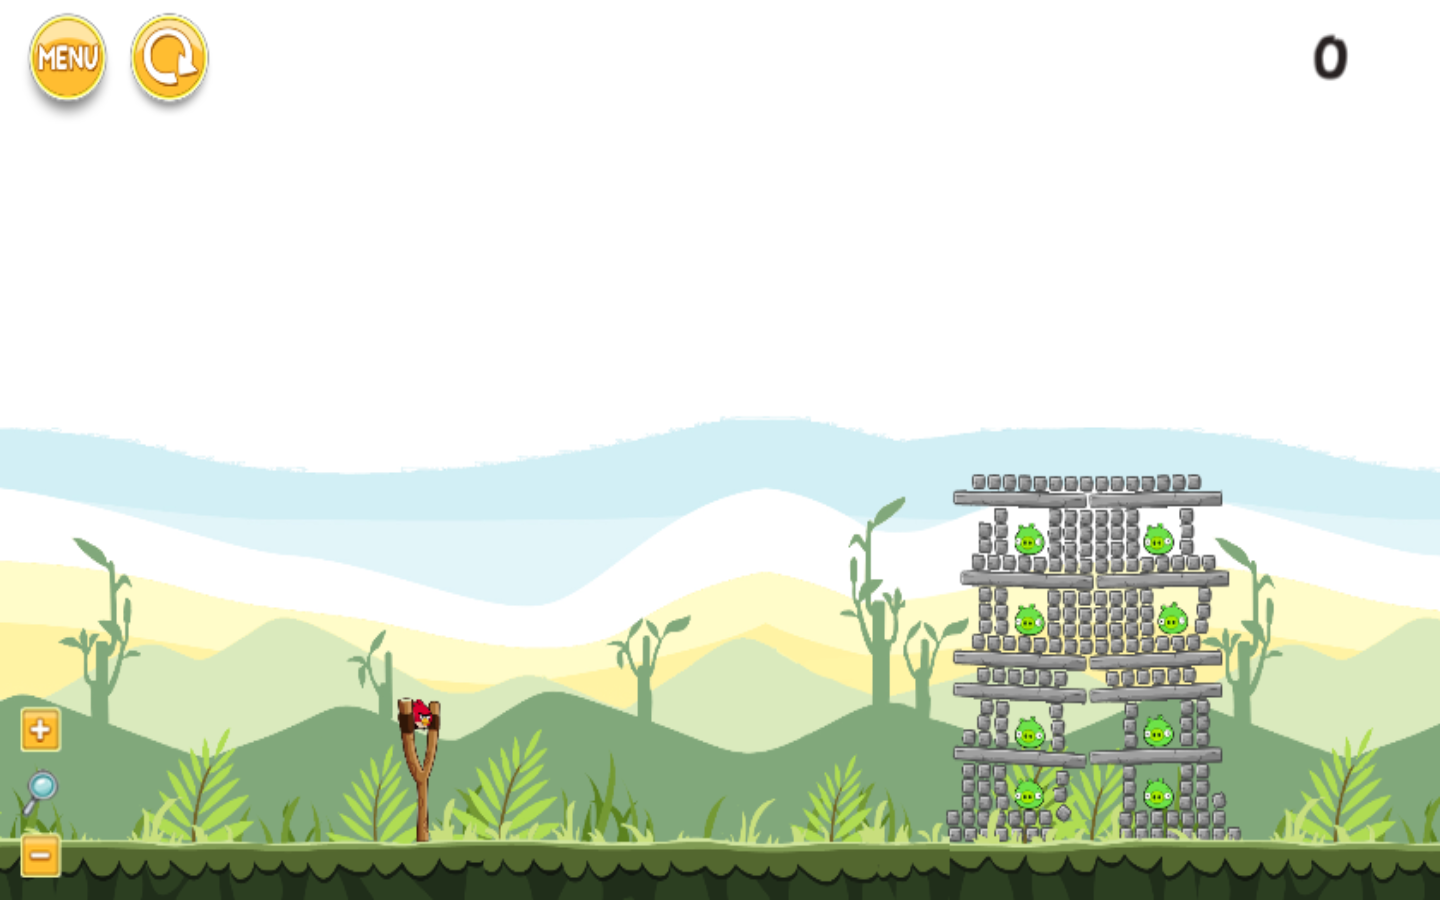
\includegraphics[width=\textwidth,height=\textheight,keepaspectratio]{levels/screenshots/buildings/triumphal_arch.png}
\end{figure}

\begin{figure}
  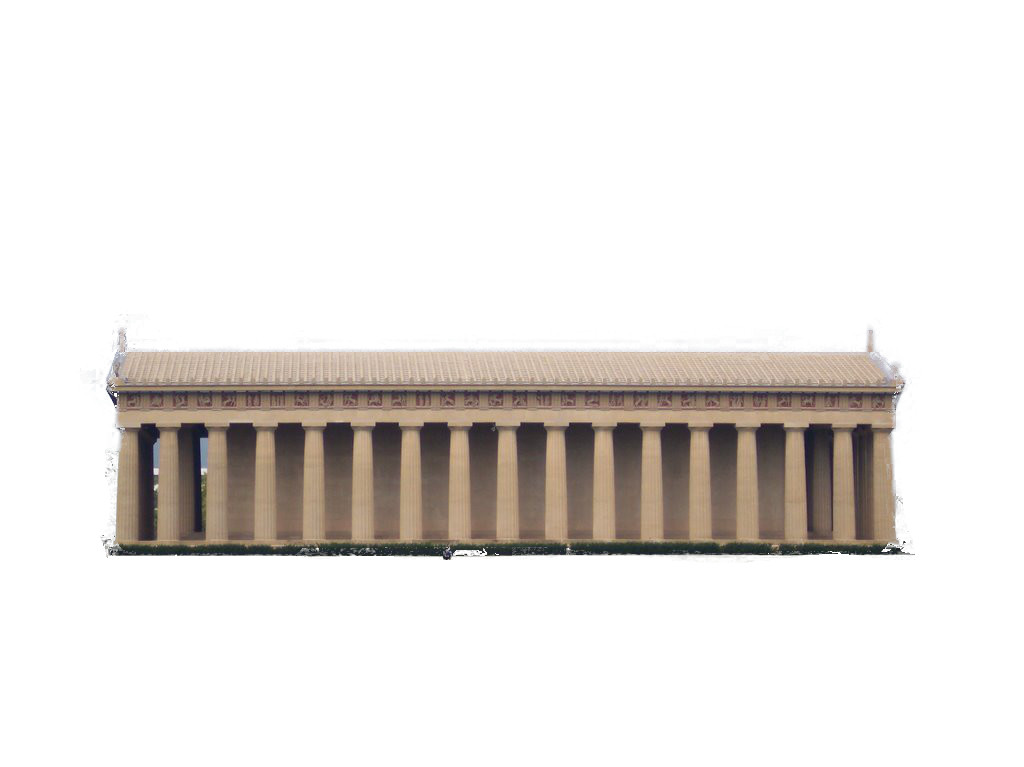
\includegraphics[width=\textwidth,height=\textheight,keepaspectratio]{levels/pictures/buildings/parthenon.jpg}
  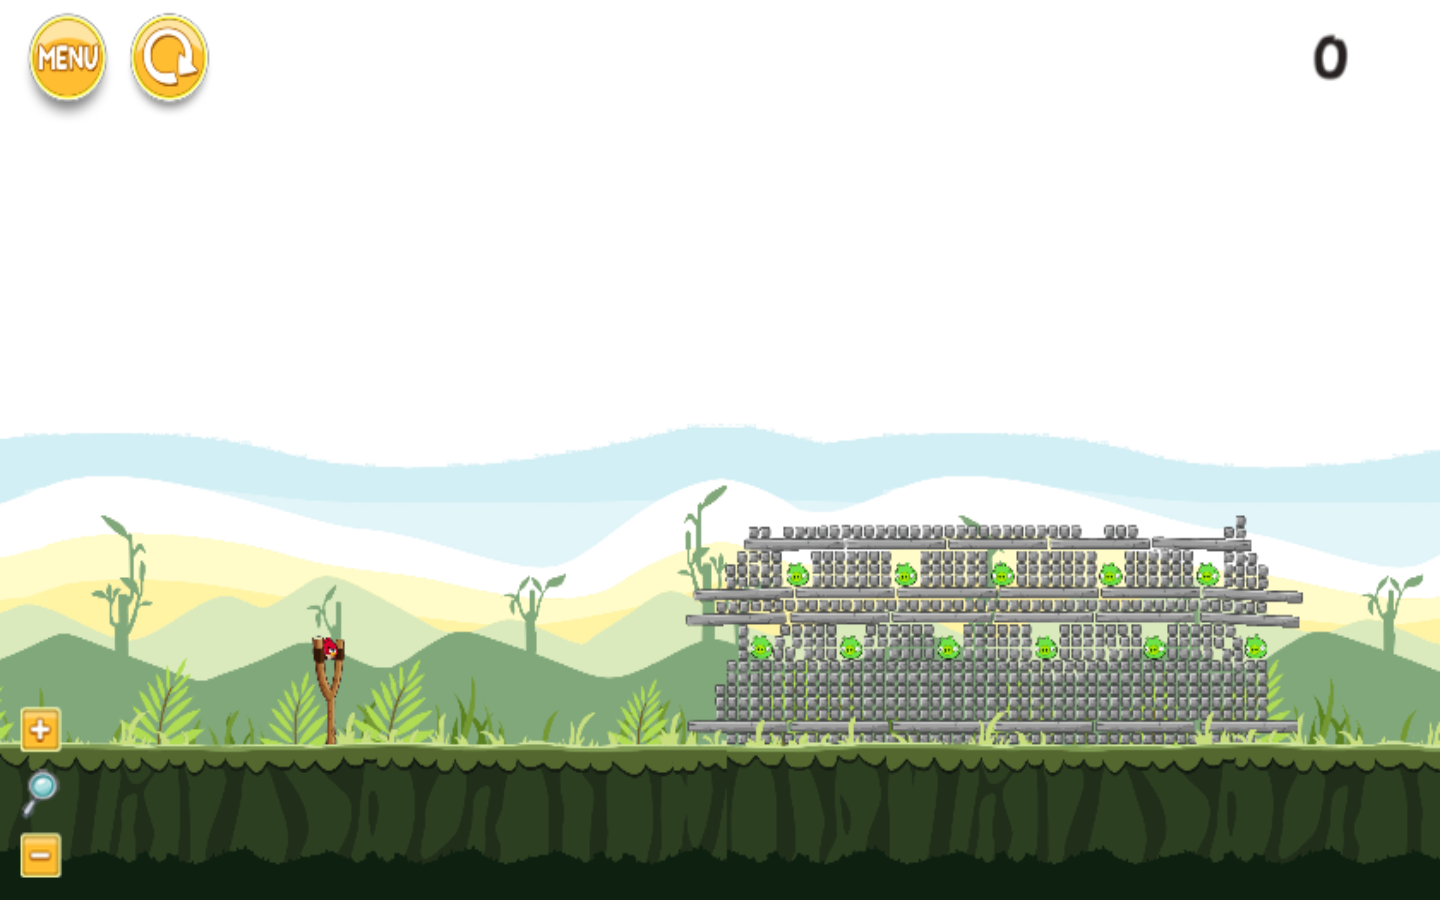
\includegraphics[width=\textwidth,height=\textheight,keepaspectratio]{levels/screenshots/buildings/parthenon.png}
\end{figure}

\begin{figure}
  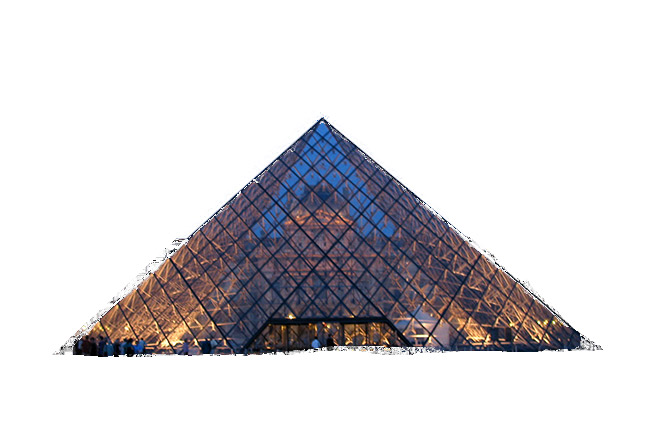
\includegraphics[width=\textwidth,height=\textheight,keepaspectratio]{levels/pictures/buildings/louvre_pyramid.jpg}
  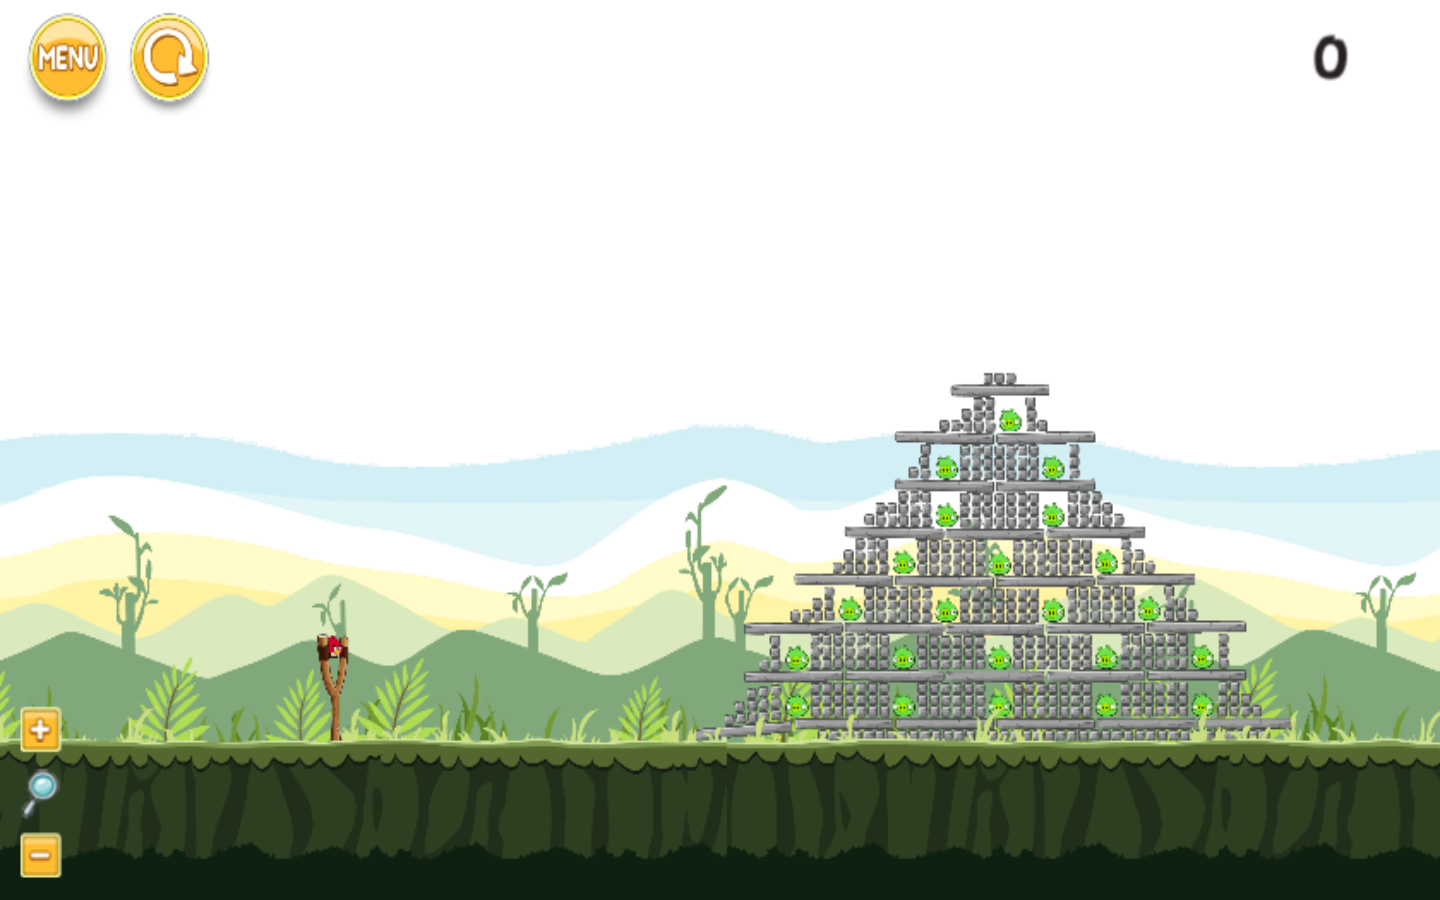
\includegraphics[width=\textwidth,height=\textheight,keepaspectratio]{levels/screenshots/buildings/louvre_pyramid.png}
\end{figure}

\begin{figure}
  
\includegraphics[width=\textwidth,height=\textheight,keepaspectratio]{levels/pictures/halloween/grime.jpg}
  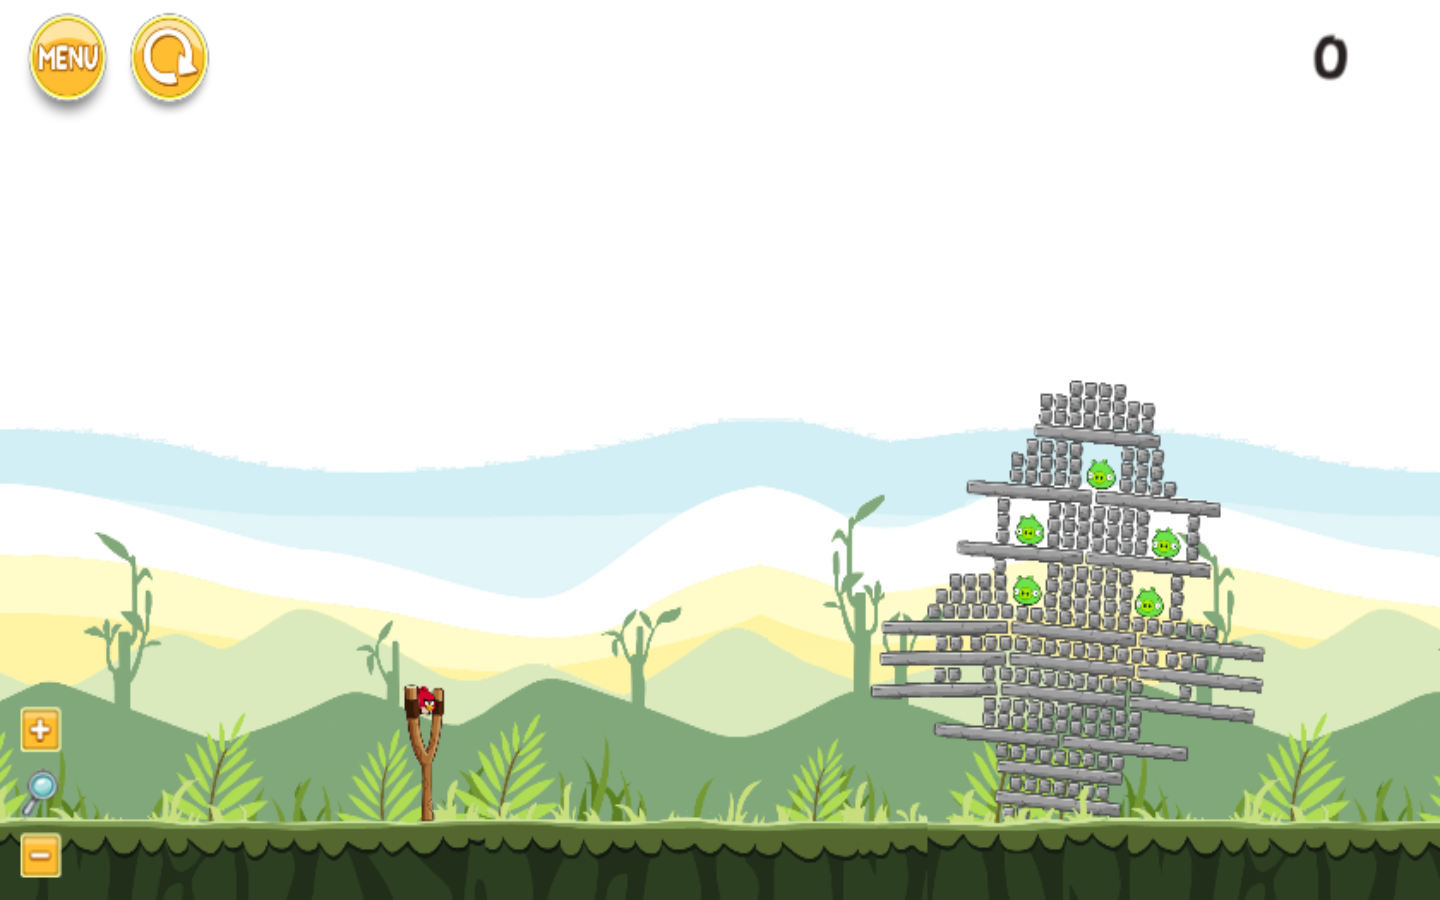
\includegraphics[width=\textwidth,height=\textheight,keepaspectratio]{levels/screenshots/halloween/grime.png}
\end{figure}

\begin{figure}
  
\includegraphics[width=\textwidth,height=\textheight,keepaspectratio]{levels/pictures/halloween/jack_o_lantern.jpg}
  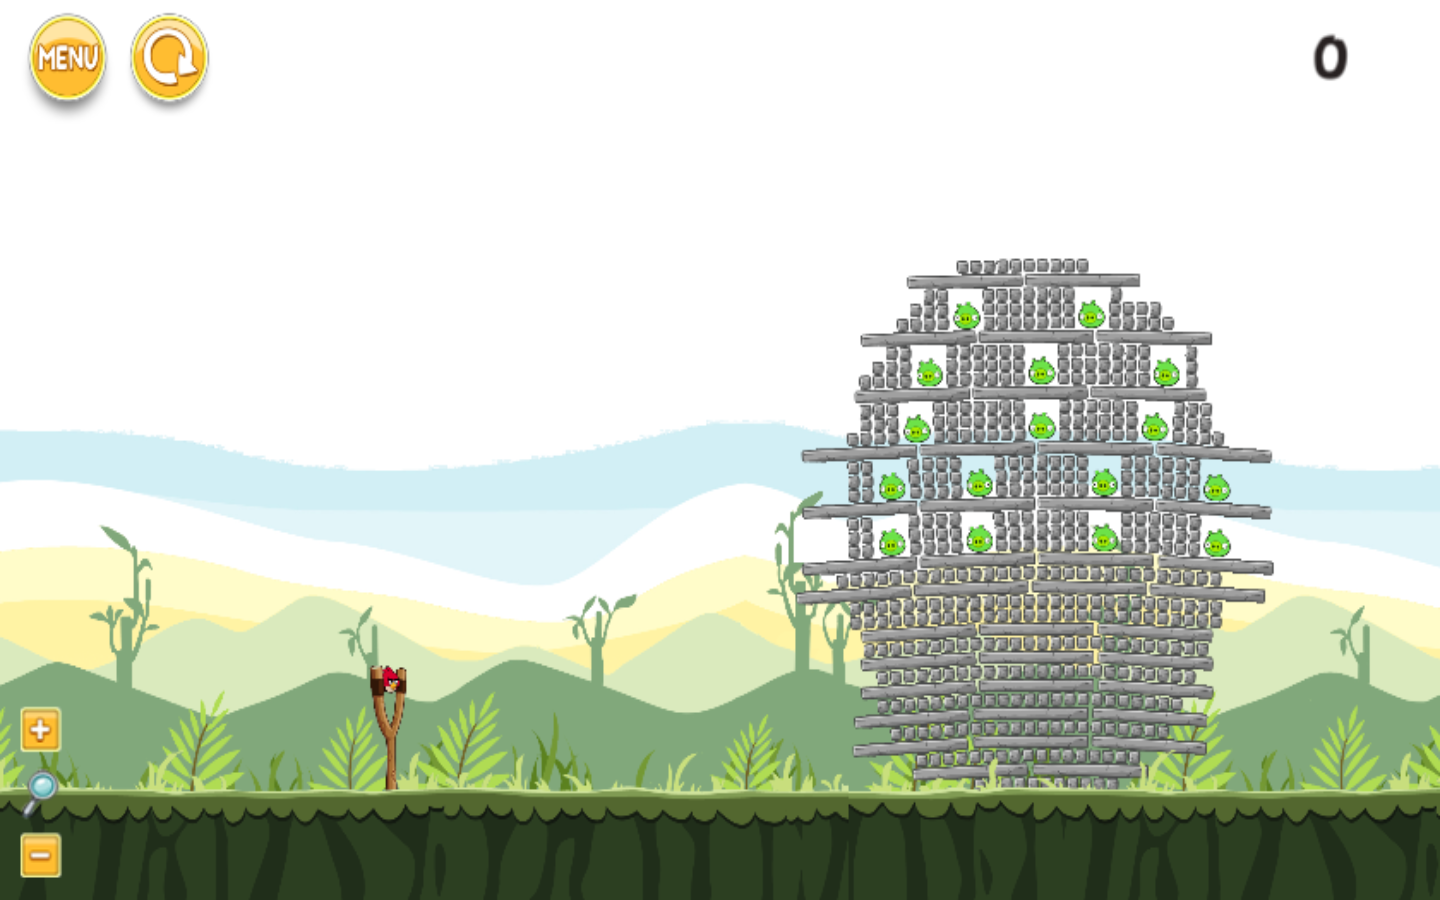
\includegraphics[width=\textwidth,height=\textheight,keepaspectratio]{levels/screenshots/halloween/jack_o_lantern.png}
\end{figure}

\begin{figure}
  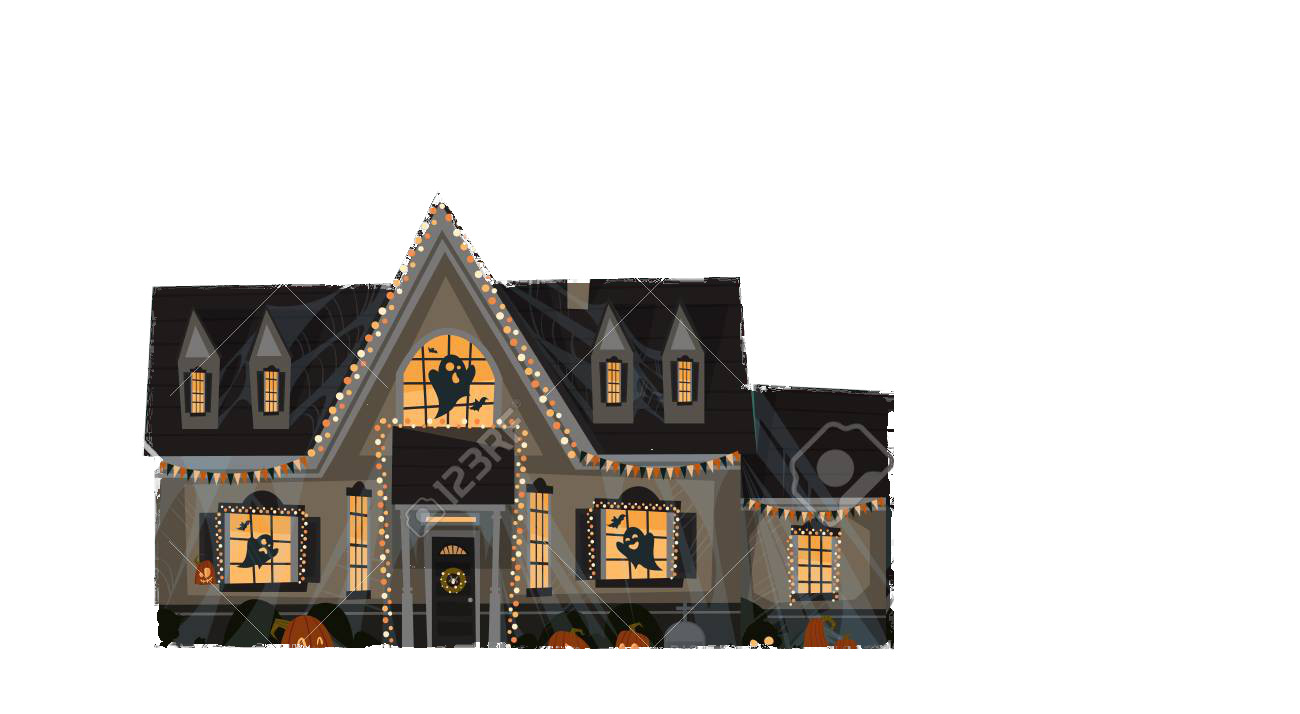
\includegraphics[width=\textwidth,height=\textheight,keepaspectratio]{levels/pictures/halloween/haunted_house.jpg}
  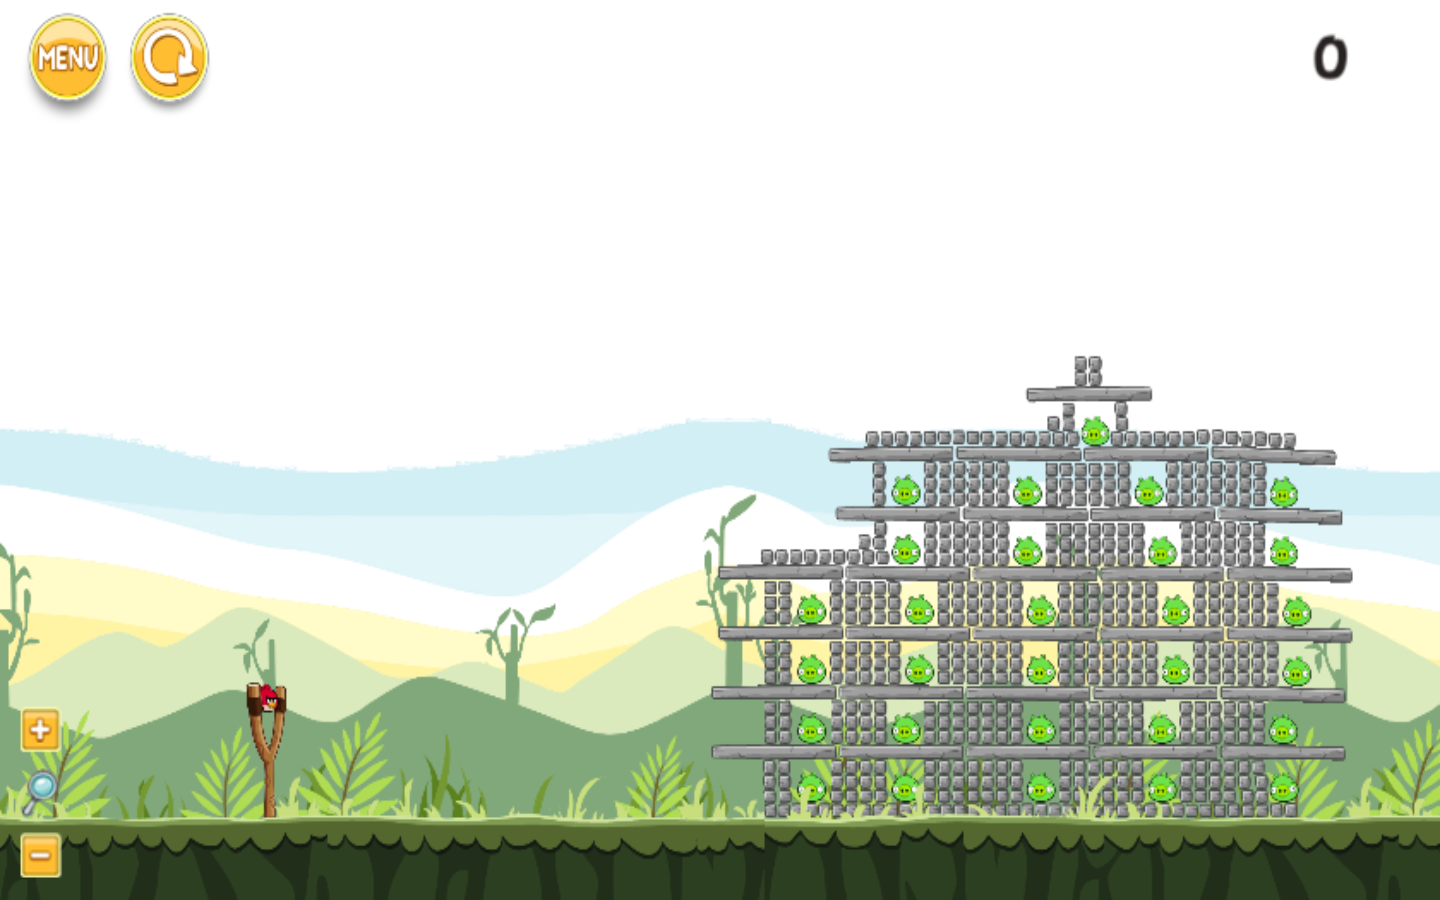
\includegraphics[width=\textwidth,height=\textheight,keepaspectratio]{levels/screenshots/halloween/haunted_house.png}
\end{figure}

\begin{figure}
  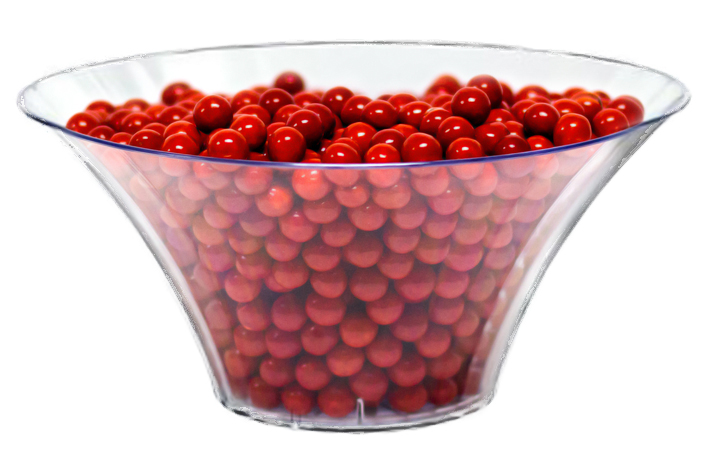
\includegraphics[width=\textwidth,height=\textheight,keepaspectratio]{levels/pictures/halloween/candy_bowl.jpg}
  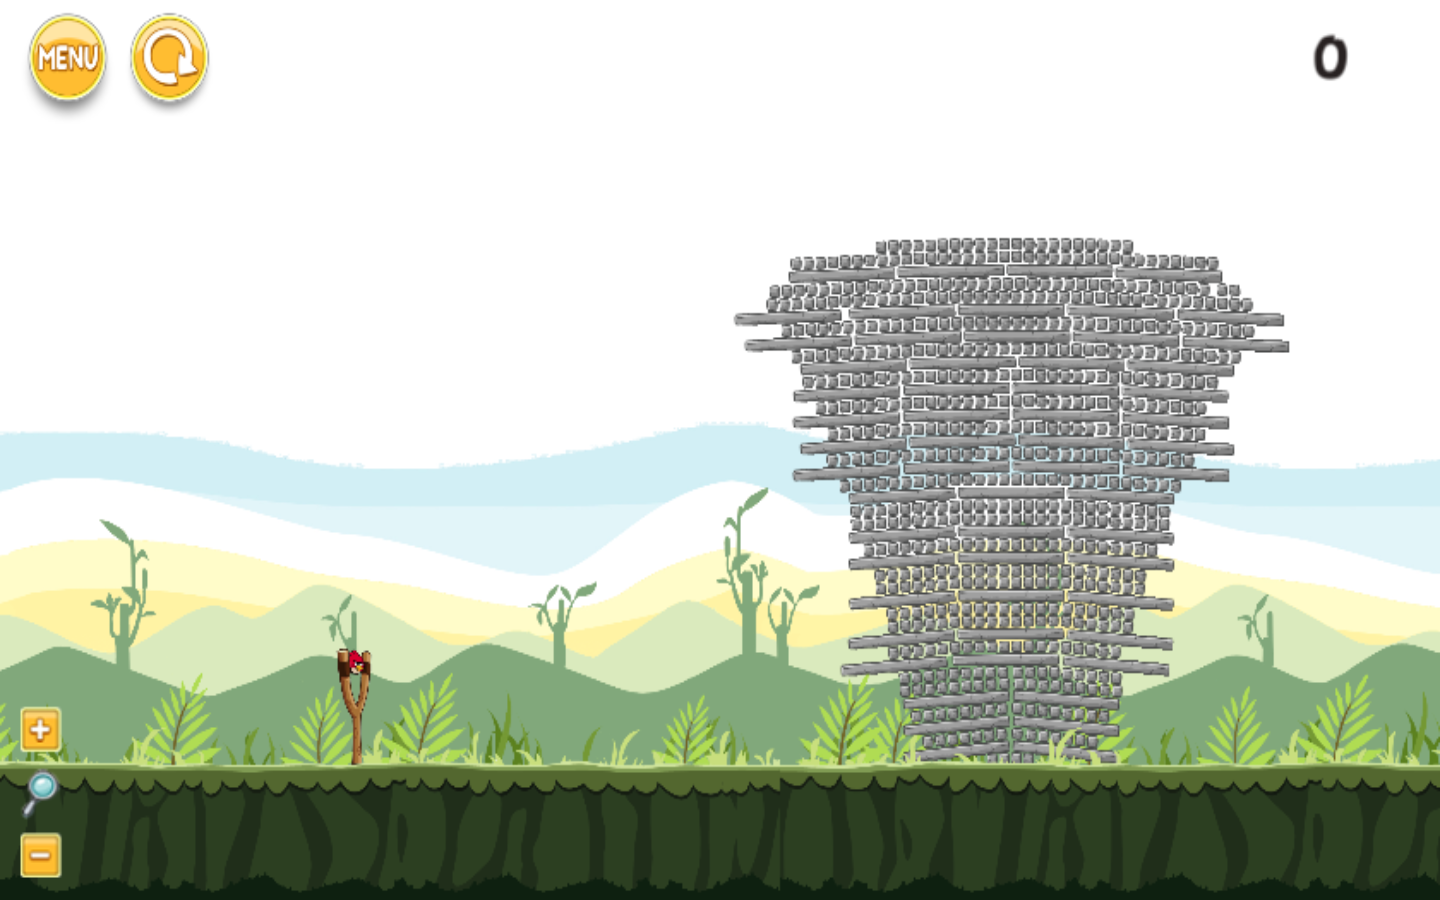
\includegraphics[width=\textwidth,height=\textheight,keepaspectratio]{levels/screenshots/halloween/candy_bowl.png}
\end{figure}

\begin{figure}
  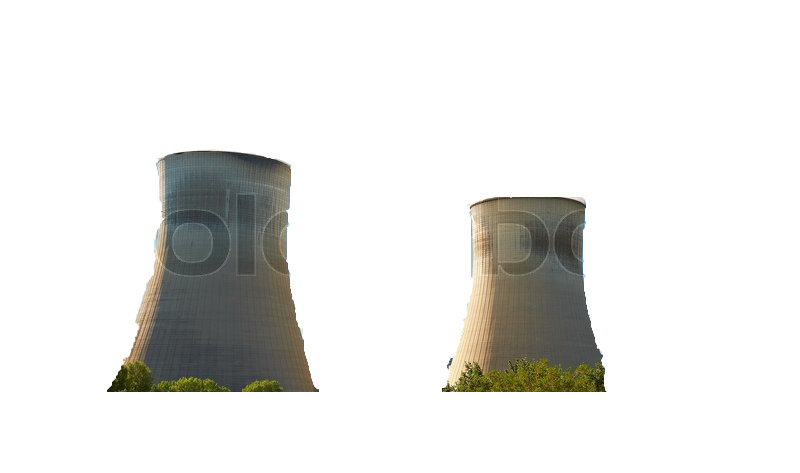
\includegraphics[width=\textwidth,height=\textheight,keepaspectratio]{levels/pictures/mechanisms/chimneys.jpg}
  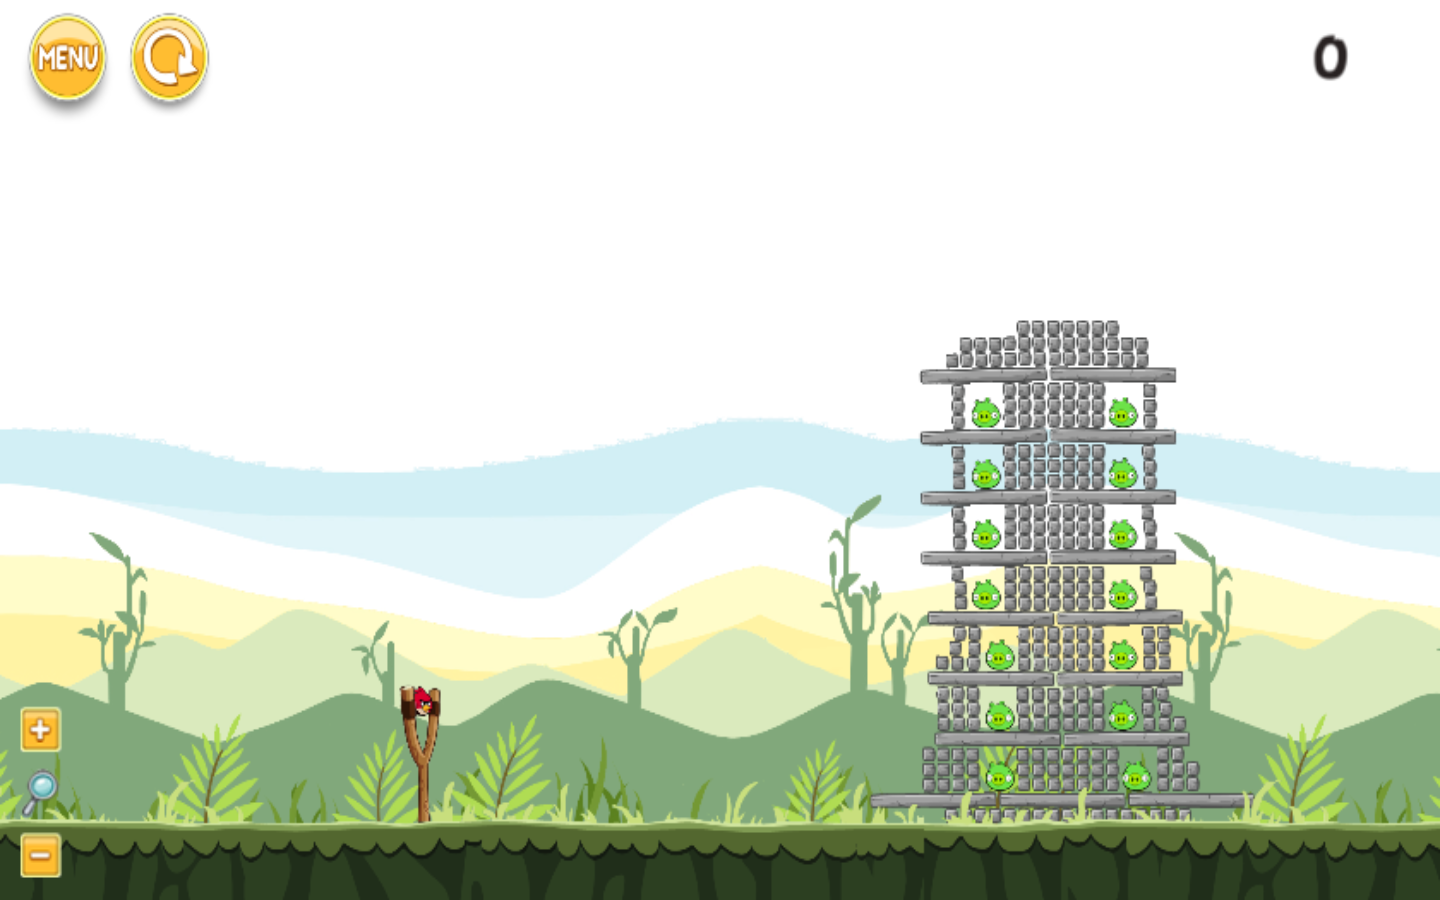
\includegraphics[width=\textwidth,height=\textheight,keepaspectratio]{levels/screenshots/mechanisms/chimneys.png}
\end{figure}

\begin{figure}
  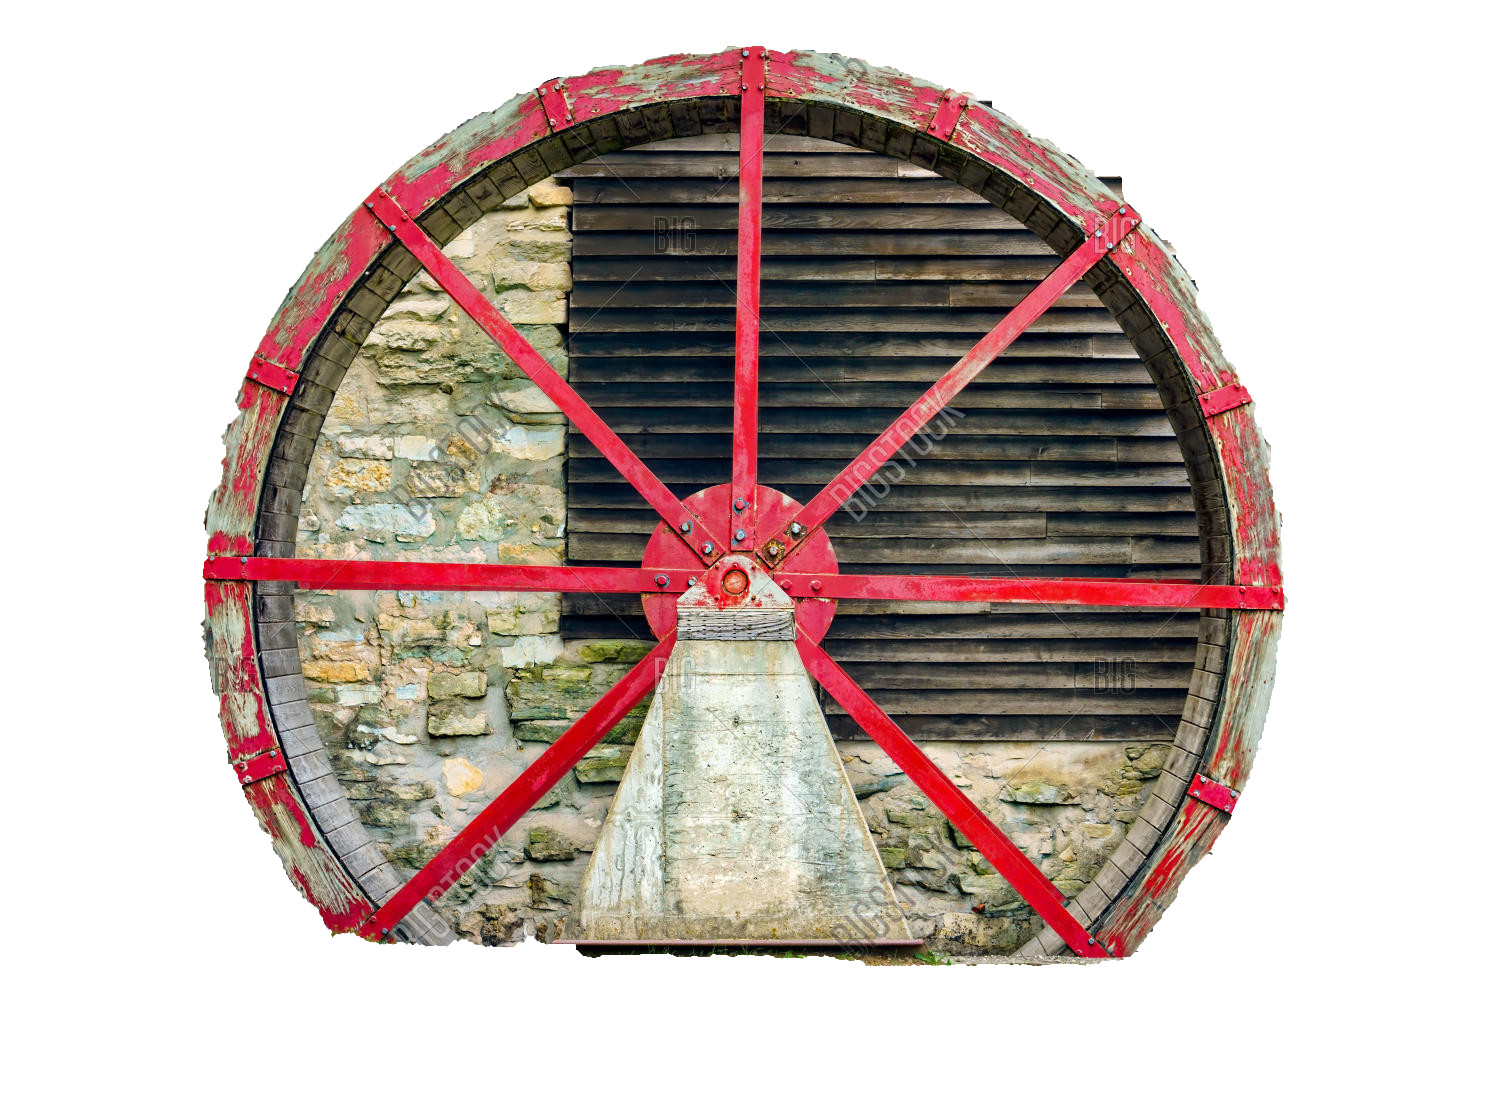
\includegraphics[width=\textwidth,height=\textheight,keepaspectratio]{levels/pictures/mechanisms/water_wheel.jpg}
  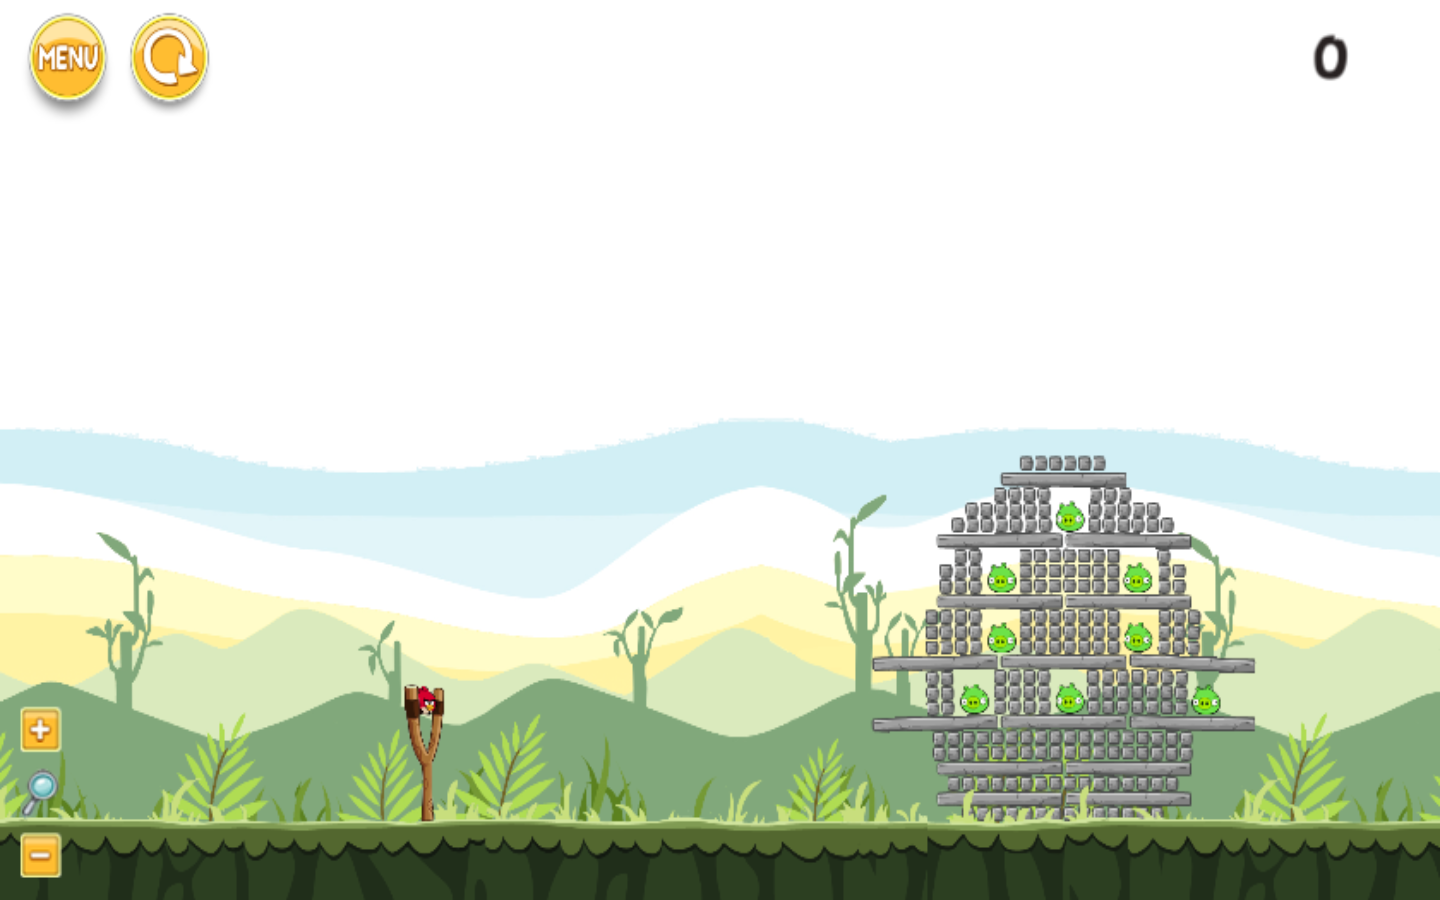
\includegraphics[width=\textwidth,height=\textheight,keepaspectratio]{levels/screenshots/mechanisms/water_wheel.png}
\end{figure}

\begin{figure}
  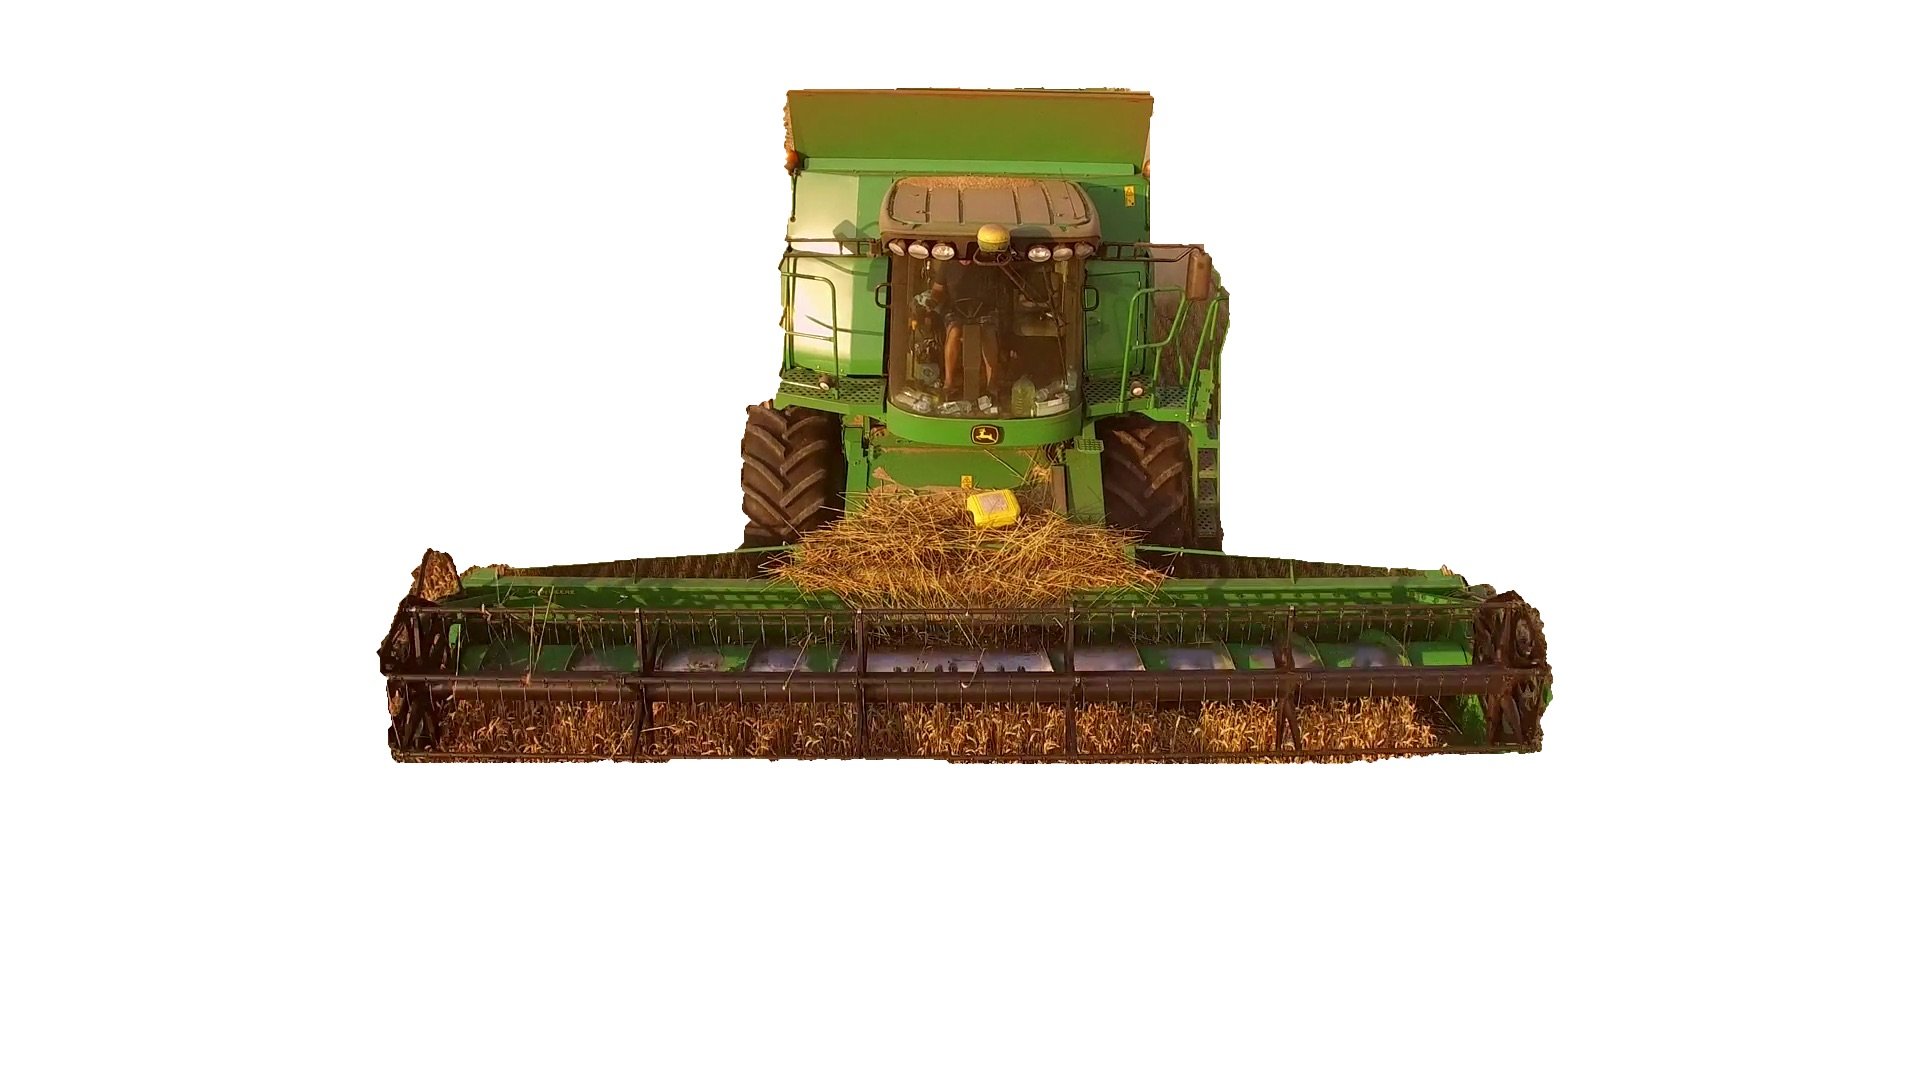
\includegraphics[width=\textwidth,height=\textheight,keepaspectratio]{levels/pictures/mechanisms/combine_harvester.jpg}
  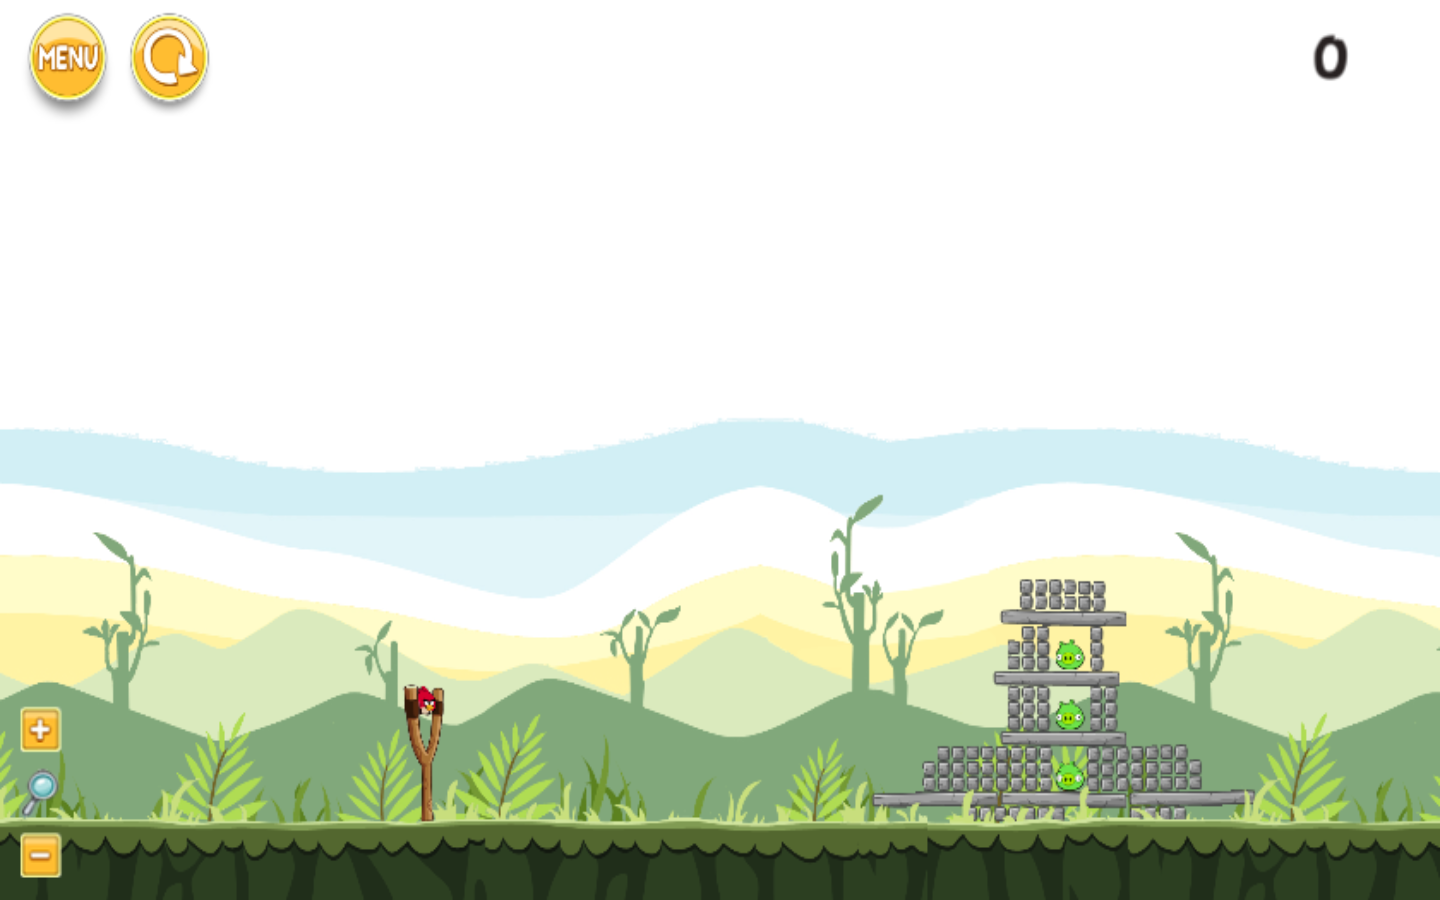
\includegraphics[width=\textwidth,height=\textheight,keepaspectratio]{levels/screenshots/mechanisms/combine_harvester.png}
\end{figure}

\begin{figure}
  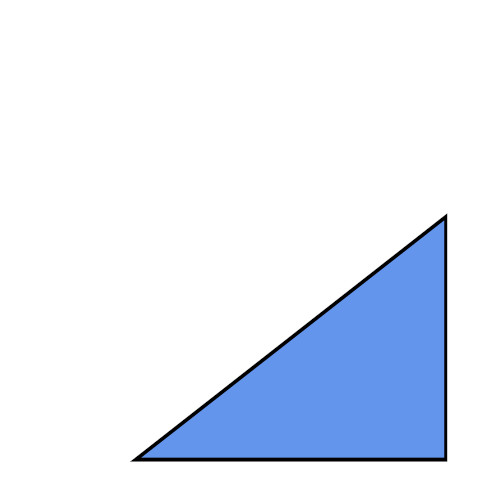
\includegraphics[width=\textwidth,height=\textheight,keepaspectratio]{levels/pictures/mechanisms/inclined_plane.jpg}
  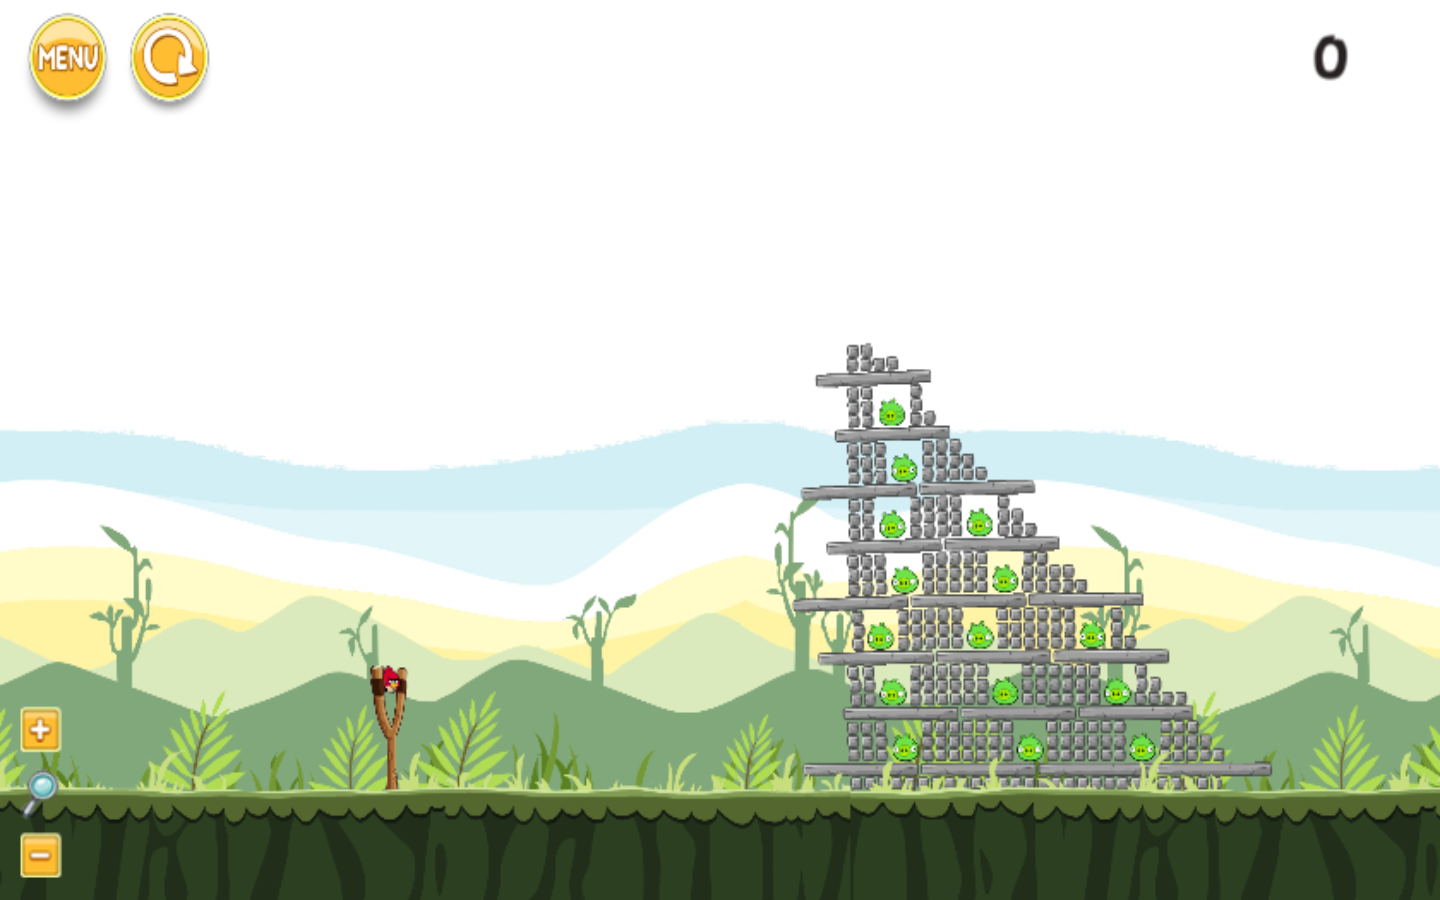
\includegraphics[width=\textwidth,height=\textheight,keepaspectratio]{levels/screenshots/mechanisms/inclined_plane.png}
\end{figure}

\begin{figure}
  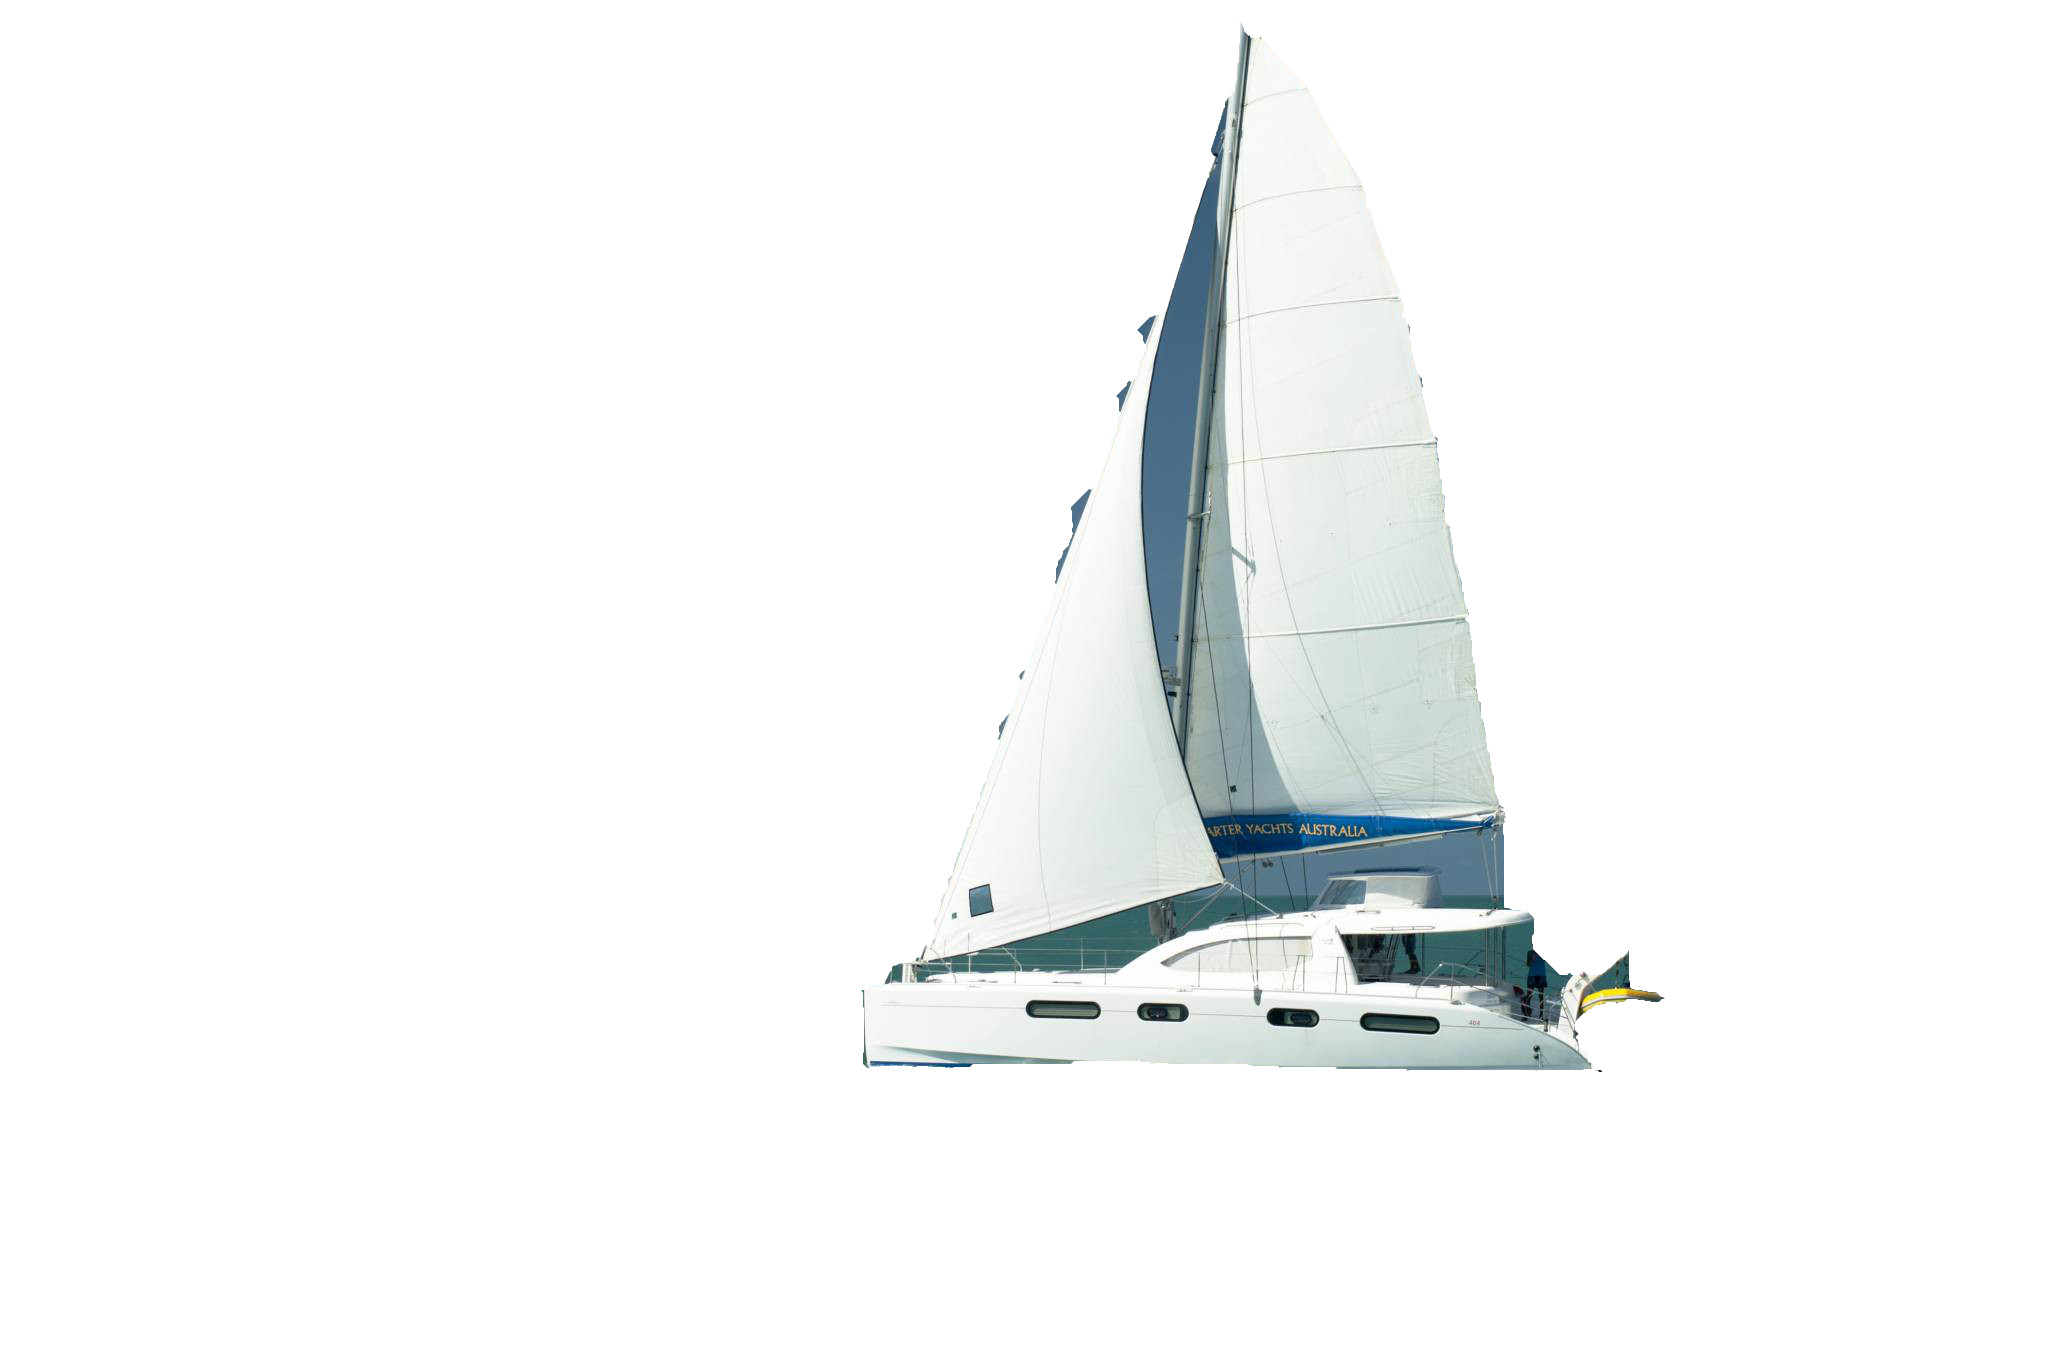
\includegraphics[width=\textwidth,height=\textheight,keepaspectratio]{levels/pictures/ships/catamaran.jpg}
  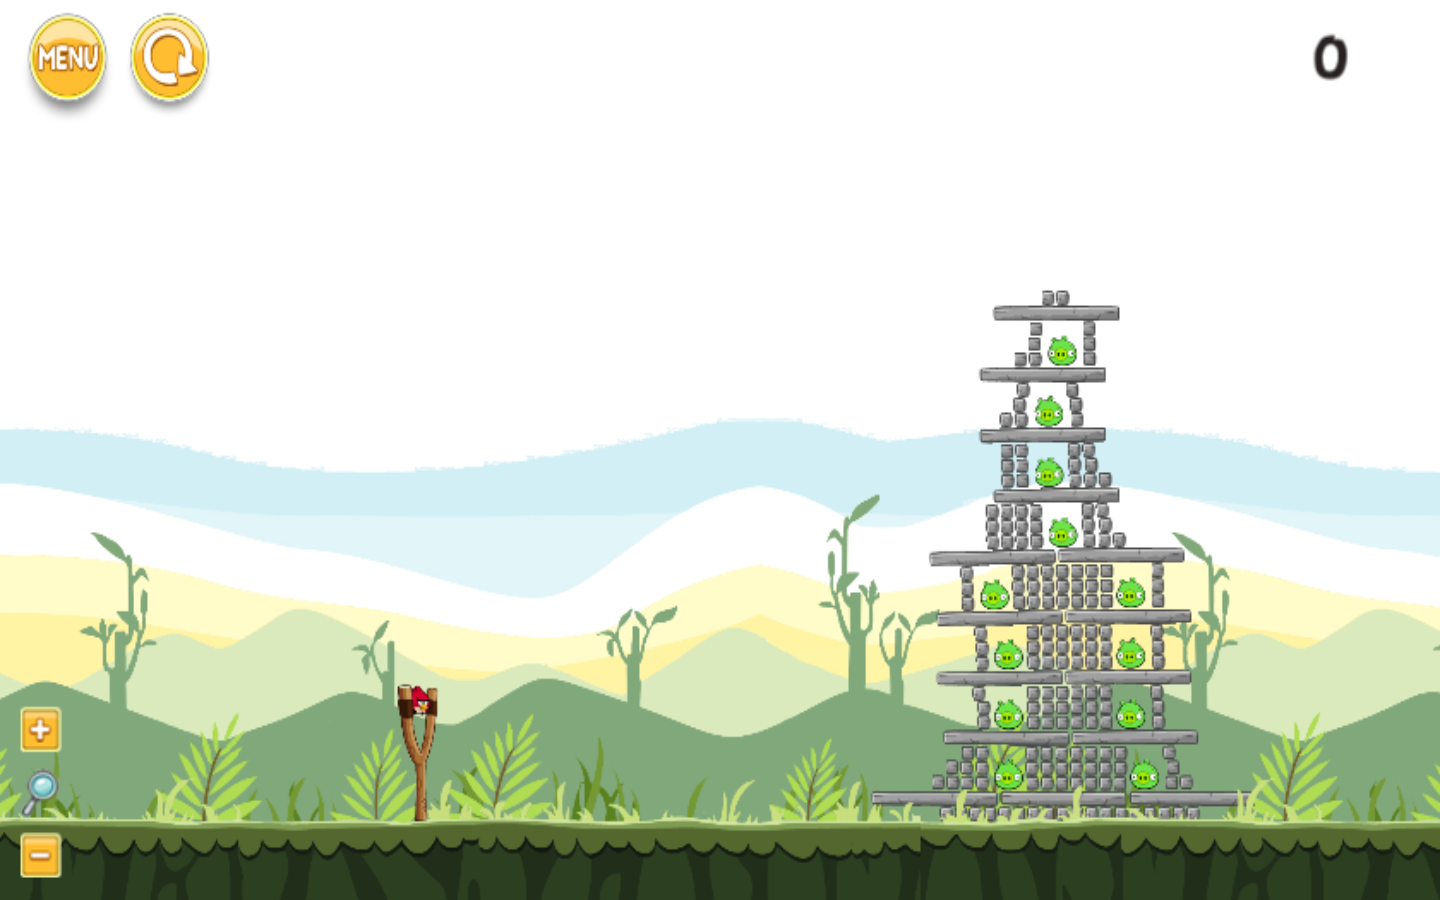
\includegraphics[width=\textwidth,height=\textheight,keepaspectratio]{levels/screenshots/ships/catamaran.png}
\end{figure}

\begin{figure}
  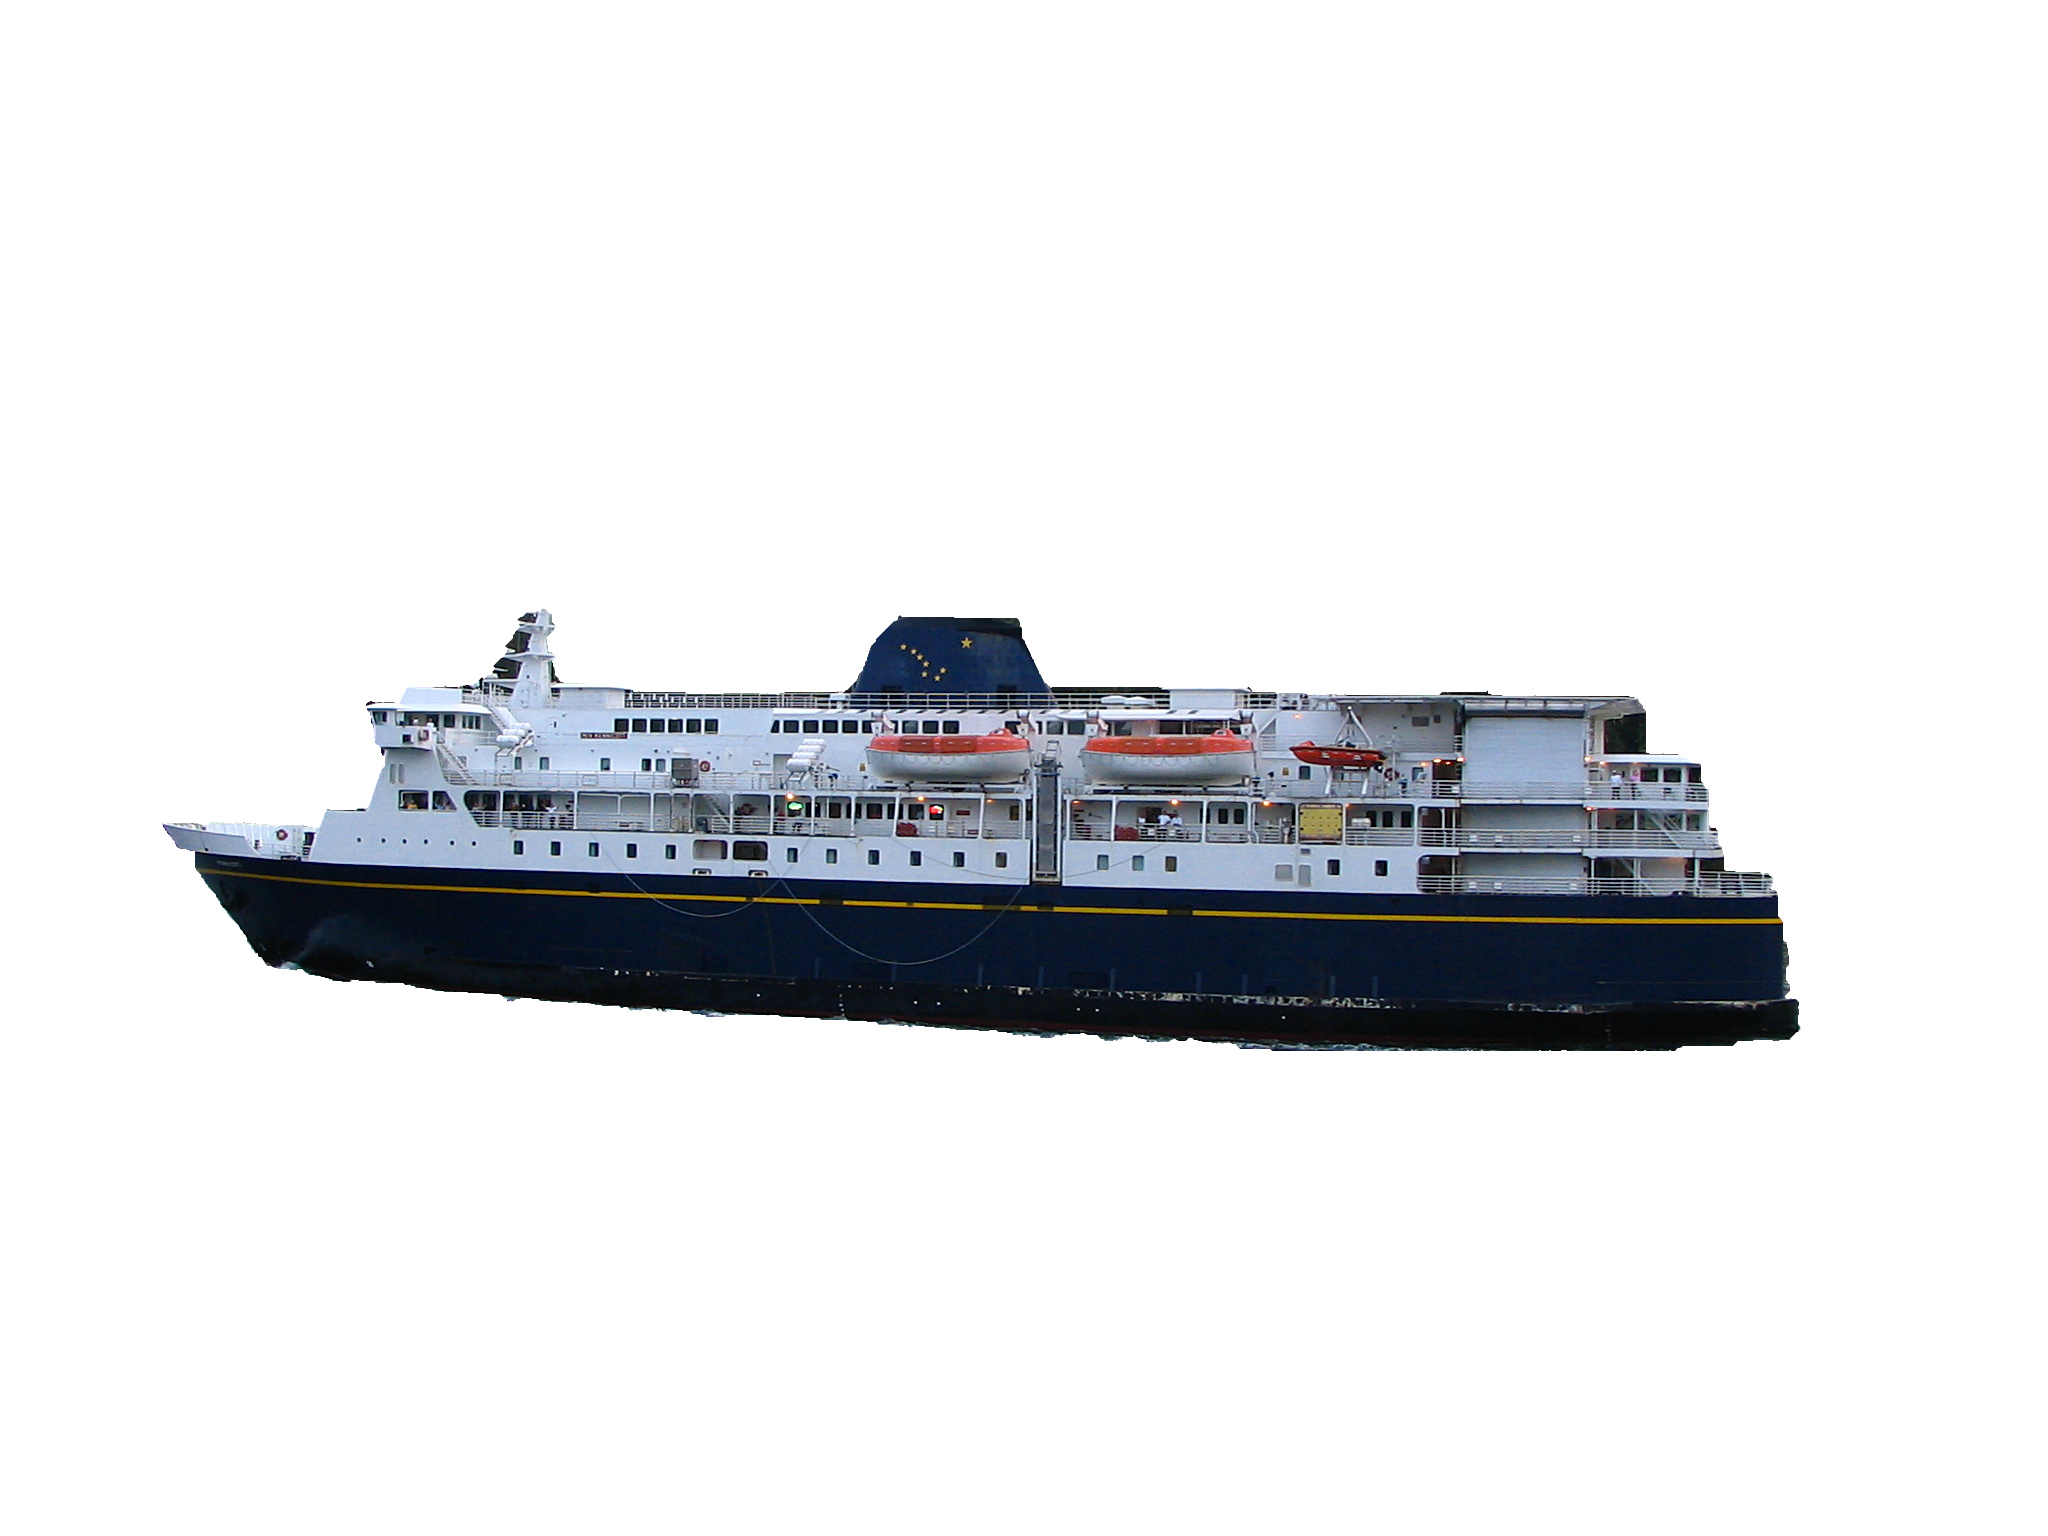
\includegraphics[width=\textwidth,height=\textheight,keepaspectratio]{levels/pictures/ships/ferry.jpg}
  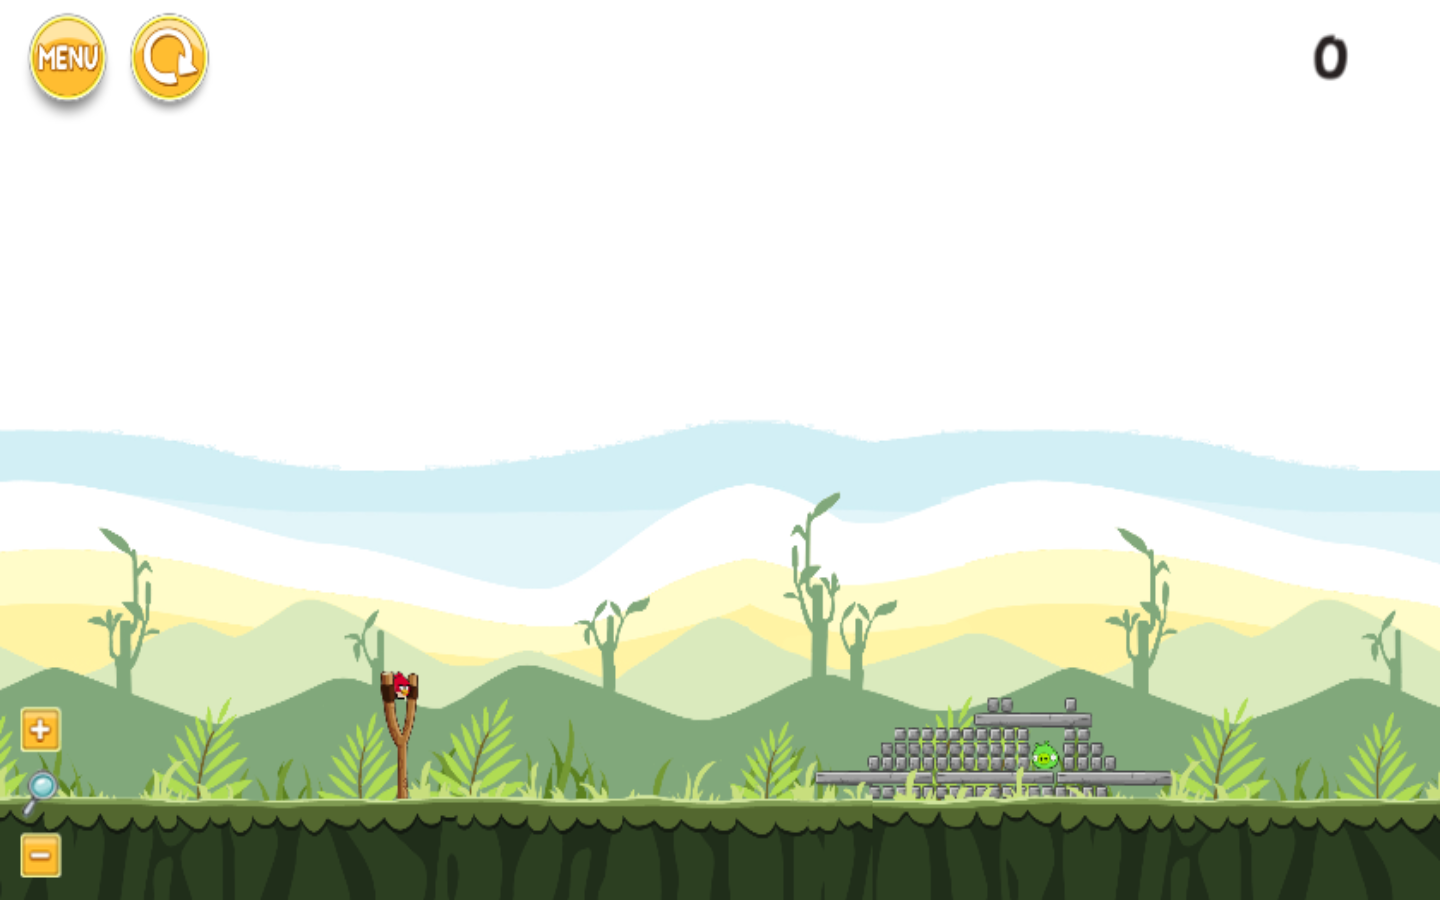
\includegraphics[width=\textwidth,height=\textheight,keepaspectratio]{levels/screenshots/ships/ferry.png}
\end{figure}

\begin{figure}
  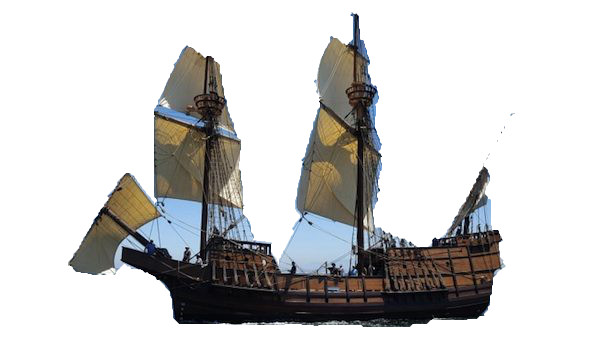
\includegraphics[width=\textwidth,height=\textheight,keepaspectratio]{levels/pictures/ships/galleon.jpg}
  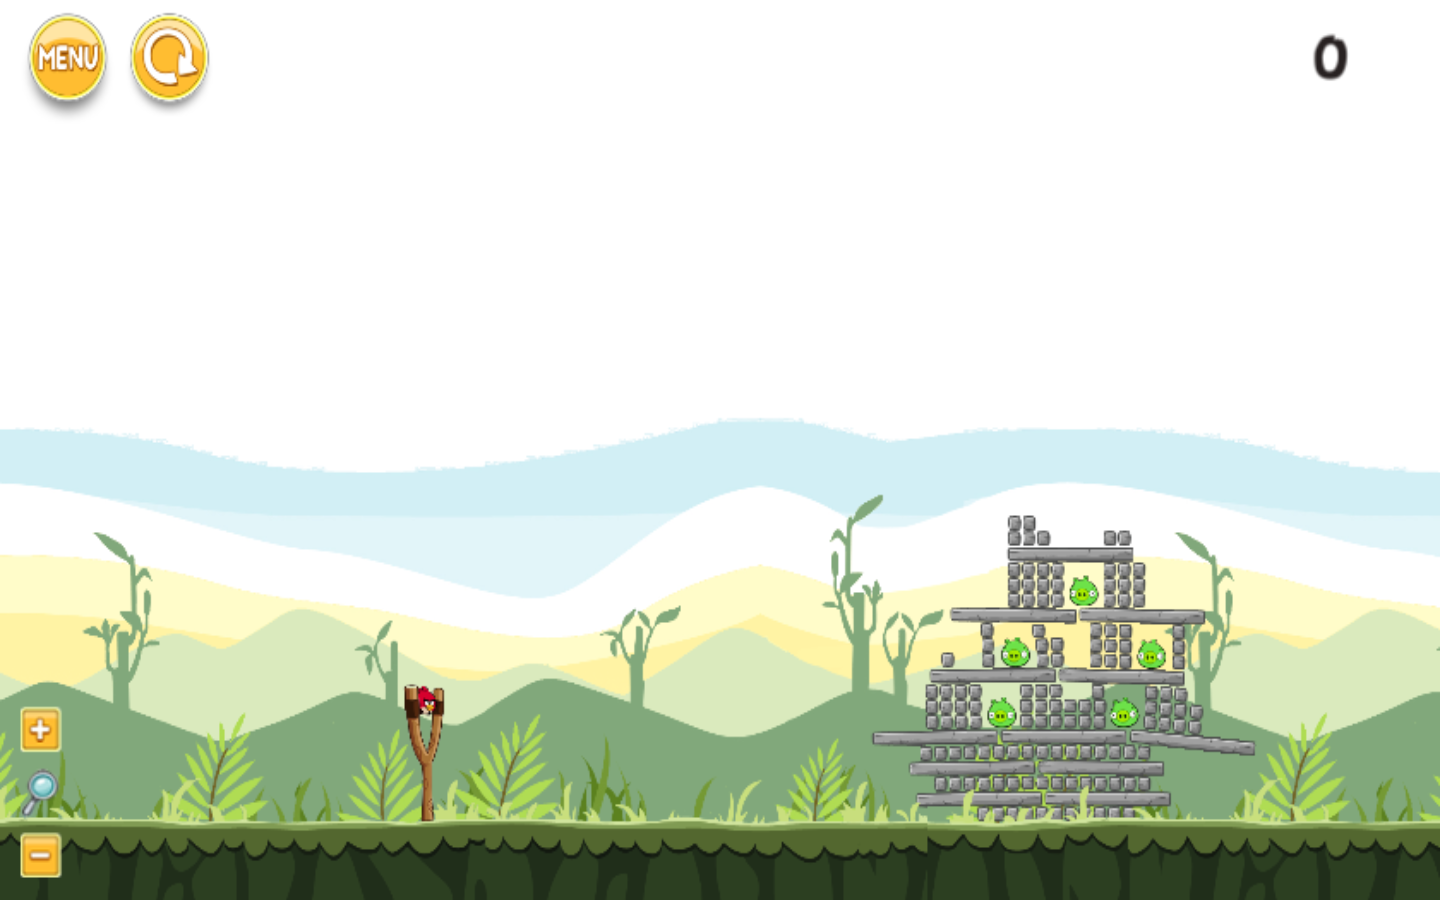
\includegraphics[width=\textwidth,height=\textheight,keepaspectratio]{levels/screenshots/ships/galleon.png}
\end{figure}

\begin{figure}
  \includegraphics[width=\textwidth,height=\textheight,keepaspectratio]{levels/pictures/ships/rowboat.jpg}
  \includegraphics[width=\textwidth,height=\textheight,keepaspectratio]{levels/screenshots/ships/rowboat.png}
\end{figure}

\end{document}
